\documentclass[twoside]{book}

% Packages required by doxygen
\usepackage{calc}
\usepackage{doxygen}
\usepackage{graphicx}
\usepackage[utf8]{inputenc}
\usepackage{makeidx}
\usepackage{multicol}
\usepackage{multirow}
\usepackage{textcomp}
\usepackage[table]{xcolor}

% NLS support packages
Portuguese
% Font selection
\usepackage[T1]{fontenc}
\usepackage{mathptmx}
\usepackage[scaled=.90]{helvet}
\usepackage{courier}
\usepackage{amssymb}
\usepackage{sectsty}
\renewcommand{\familydefault}{\sfdefault}
\allsectionsfont{%
  \fontseries{bc}\selectfont%
  \color{darkgray}%
}
\renewcommand{\DoxyLabelFont}{%
  \fontseries{bc}\selectfont%
  \color{darkgray}%
}

% Page & text layout
\usepackage{geometry}
\geometry{%
  a4paper,%
  top=2.5cm,%
  bottom=2.5cm,%
  left=2.5cm,%
  right=2.5cm%
}
\tolerance=750
\hfuzz=15pt
\hbadness=750
\setlength{\emergencystretch}{15pt}
\setlength{\parindent}{0cm}
\setlength{\parskip}{0.2cm}
\makeatletter
\renewcommand{\paragraph}{%
  \@startsection{paragraph}{4}{0ex}{-1.0ex}{1.0ex}{%
    \normalfont\normalsize\bfseries\SS@parafont%
  }%
}
\renewcommand{\subparagraph}{%
  \@startsection{subparagraph}{5}{0ex}{-1.0ex}{1.0ex}{%
    \normalfont\normalsize\bfseries\SS@subparafont%
  }%
}
\makeatother

% Headers & footers
\usepackage{fancyhdr}
\pagestyle{fancyplain}
\fancyhead[LE]{\fancyplain{}{\bfseries\thepage}}
\fancyhead[CE]{\fancyplain{}{}}
\fancyhead[RE]{\fancyplain{}{\bfseries\leftmark}}
\fancyhead[LO]{\fancyplain{}{\bfseries\rightmark}}
\fancyhead[CO]{\fancyplain{}{}}
\fancyhead[RO]{\fancyplain{}{\bfseries\thepage}}
\fancyfoot[LE]{\fancyplain{}{}}
\fancyfoot[CE]{\fancyplain{}{}}
\fancyfoot[RE]{\fancyplain{}{\bfseries\scriptsize Gerado em Sexta, 17 de Junho de 2016 22\-:23\-:22 para Projeto Final M\-P por Doxygen }}
\fancyfoot[LO]{\fancyplain{}{\bfseries\scriptsize Gerado em Sexta, 17 de Junho de 2016 22\-:23\-:22 para Projeto Final M\-P por Doxygen }}
\fancyfoot[CO]{\fancyplain{}{}}
\fancyfoot[RO]{\fancyplain{}{}}
\renewcommand{\footrulewidth}{0.4pt}
\renewcommand{\chaptermark}[1]{%
  \markboth{#1}{}%
}
\renewcommand{\sectionmark}[1]{%
  \markright{\thesection\ #1}%
}

% Indices & bibliography
\usepackage{natbib}
\usepackage[titles]{tocloft}
\setcounter{tocdepth}{3}
\setcounter{secnumdepth}{5}
\makeindex

% Hyperlinks (required, but should be loaded last)
\usepackage{ifpdf}
\ifpdf
  \usepackage[pdftex,pagebackref=true]{hyperref}
\else
  \usepackage[ps2pdf,pagebackref=true]{hyperref}
\fi
\hypersetup{%
  colorlinks=true,%
  linkcolor=blue,%
  citecolor=blue,%
  unicode%
}

% Custom commands
\newcommand{\clearemptydoublepage}{%
  \newpage{\pagestyle{empty}\cleardoublepage}%
}


%===== C O N T E N T S =====

\begin{document}

% Titlepage & ToC
\hypersetup{pageanchor=false}
\pagenumbering{roman}
\begin{titlepage}
\vspace*{7cm}
\begin{center}%
{\Large Projeto Final M\-P }\\
\vspace*{1cm}
{\large Gerado por Doxygen 1.8.6}\\
\vspace*{0.5cm}
{\small Sexta, 17 de Junho de 2016 22:23:22}\\
\end{center}
\end{titlepage}
\clearemptydoublepage
\tableofcontents
\clearemptydoublepage
\pagenumbering{arabic}
\hypersetup{pageanchor=true}

%--- Begin generated contents ---
\chapter{Índice dos componentes}
\section{Lista de componentes}
Lista de classes, estruturas, uniões e interfaces com uma breve descrição\-:\begin{DoxyCompactList}
\item\contentsline{section}{\hyperlink{structGrafo}{Grafo} }{\pageref{structGrafo}}{}
\item\contentsline{section}{\hyperlink{structLISTA}{L\-I\-S\-T\-A} }{\pageref{structLISTA}}{}
\item\contentsline{section}{\hyperlink{structPreRequisitos}{Pre\-Requisitos} }{\pageref{structPreRequisitos}}{}
\item\contentsline{section}{\hyperlink{structTarefa}{Tarefa} }{\pageref{structTarefa}}{}
\item\contentsline{section}{\hyperlink{structvetor}{vetor} }{\pageref{structvetor}}{}
\end{DoxyCompactList}

\chapter{Índice dos ficheiros}
\section{Lista de ficheiros}
Lista de todos os ficheiros com uma breve descrição\-:\begin{DoxyCompactList}
\item\contentsline{section}{code/\hyperlink{grafo_8cc}{grafo.\-cc} }{\pageref{grafo_8cc}}{}
\item\contentsline{section}{code/\hyperlink{gtest__grafo_8cc}{gtest\-\_\-grafo.\-cc} }{\pageref{gtest__grafo_8cc}}{}
\item\contentsline{section}{code/\hyperlink{main_8cc}{main.\-cc} }{\pageref{main_8cc}}{}
\item\contentsline{section}{include/\hyperlink{grafo_8h}{grafo.\-h} }{\pageref{grafo_8h}}{}
\end{DoxyCompactList}

\chapter{Documentação da classe}
\hypertarget{structGrafo}{\section{Referência à estrutura Grafo}
\label{structGrafo}\index{Grafo@{Grafo}}
}


{\ttfamily \#include $<$grafo.\-h$>$}



Diagrama de colaboração para Grafo\-:
\nopagebreak
\begin{figure}[H]
\begin{center}
\leavevmode
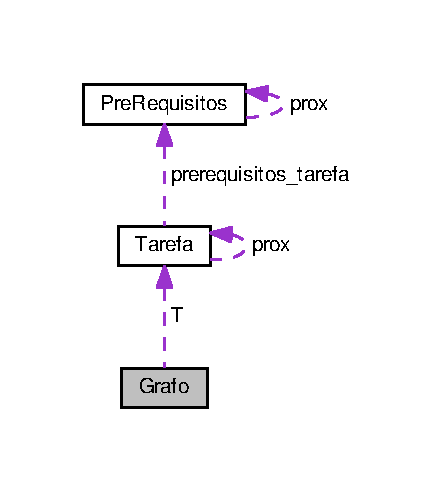
\includegraphics[width=208pt]{structGrafo__coll__graph}
\end{center}
\end{figure}
\subsection*{Atributos Públicos}
\begin{DoxyCompactItemize}
\item 
\hyperlink{grafo_8h_ab156210f10bb550f6d61bea964f08c22}{tarefa} $\ast$ \hyperlink{structGrafo_aeb37989f62bb38c1b5ebce8bfa63ad32}{T}
\end{DoxyCompactItemize}


\subsection{Documentação dos dados membro}
\hypertarget{structGrafo_aeb37989f62bb38c1b5ebce8bfa63ad32}{\index{Grafo@{Grafo}!T@{T}}
\index{T@{T}!Grafo@{Grafo}}
\subsubsection[{T}]{\setlength{\rightskip}{0pt plus 5cm}{\bf tarefa}$\ast$ Grafo\-::\-T}}\label{structGrafo_aeb37989f62bb38c1b5ebce8bfa63ad32}


A documentação para esta estrutura foi gerada a partir do seguinte ficheiro\-:\begin{DoxyCompactItemize}
\item 
include/\hyperlink{grafo_8h}{grafo.\-h}\end{DoxyCompactItemize}

\hypertarget{structLISTA}{\section{Referência à estrutura L\-I\-S\-T\-A}
\label{structLISTA}\index{L\-I\-S\-T\-A@{L\-I\-S\-T\-A}}
}
\subsection*{Atributos Públicos}
\begin{DoxyCompactItemize}
\item 
int \hyperlink{structLISTA_a81b29c44560db14d9d5ef75858c91a0b}{t}
\item 
struct \hyperlink{structLISTA}{L\-I\-S\-T\-A} $\ast$ \hyperlink{structLISTA_a818a9fbd5f34b29597c140c052309ea6}{prox}
\item 
struct \hyperlink{structLISTA}{L\-I\-S\-T\-A} $\ast$ \hyperlink{structLISTA_acbab5a56fa16181657e3036ffa9fca11}{ant}
\end{DoxyCompactItemize}


\subsection{Documentação dos dados membro}
\hypertarget{structLISTA_acbab5a56fa16181657e3036ffa9fca11}{\index{L\-I\-S\-T\-A@{L\-I\-S\-T\-A}!ant@{ant}}
\index{ant@{ant}!LISTA@{L\-I\-S\-T\-A}}
\subsubsection[{ant}]{\setlength{\rightskip}{0pt plus 5cm}struct {\bf L\-I\-S\-T\-A} $\ast$ L\-I\-S\-T\-A\-::ant}}\label{structLISTA_acbab5a56fa16181657e3036ffa9fca11}
\hypertarget{structLISTA_a818a9fbd5f34b29597c140c052309ea6}{\index{L\-I\-S\-T\-A@{L\-I\-S\-T\-A}!prox@{prox}}
\index{prox@{prox}!LISTA@{L\-I\-S\-T\-A}}
\subsubsection[{prox}]{\setlength{\rightskip}{0pt plus 5cm}struct {\bf L\-I\-S\-T\-A}$\ast$ L\-I\-S\-T\-A\-::prox}}\label{structLISTA_a818a9fbd5f34b29597c140c052309ea6}
\hypertarget{structLISTA_a81b29c44560db14d9d5ef75858c91a0b}{\index{L\-I\-S\-T\-A@{L\-I\-S\-T\-A}!t@{t}}
\index{t@{t}!LISTA@{L\-I\-S\-T\-A}}
\subsubsection[{t}]{\setlength{\rightskip}{0pt plus 5cm}int L\-I\-S\-T\-A\-::t}}\label{structLISTA_a81b29c44560db14d9d5ef75858c91a0b}


A documentação para esta estrutura foi gerada a partir do seguinte ficheiro\-:\begin{DoxyCompactItemize}
\item 
code/\hyperlink{grafo_8cc}{grafo.\-cc}\end{DoxyCompactItemize}

\hypertarget{structPreRequisitos}{\section{Referência à estrutura Pre\-Requisitos}
\label{structPreRequisitos}\index{Pre\-Requisitos@{Pre\-Requisitos}}
}


{\ttfamily \#include $<$grafo.\-h$>$}

\subsection*{Atributos Públicos}
\begin{DoxyCompactItemize}
\item 
int \hyperlink{structPreRequisitos_aac895640418edfa91ba7c8f01b91459e}{id\-\_\-prerequisito}
\item 
struct \hyperlink{structPreRequisitos}{Pre\-Requisitos} $\ast$ \hyperlink{structPreRequisitos_ad30378886dd7fba5247ad1c77fb395f1}{prox}
\end{DoxyCompactItemize}


\subsection{Documentação dos dados membro}
\hypertarget{structPreRequisitos_aac895640418edfa91ba7c8f01b91459e}{\index{Pre\-Requisitos@{Pre\-Requisitos}!id\-\_\-prerequisito@{id\-\_\-prerequisito}}
\index{id\-\_\-prerequisito@{id\-\_\-prerequisito}!PreRequisitos@{Pre\-Requisitos}}
\subsubsection[{id\-\_\-prerequisito}]{\setlength{\rightskip}{0pt plus 5cm}int Pre\-Requisitos\-::id\-\_\-prerequisito}}\label{structPreRequisitos_aac895640418edfa91ba7c8f01b91459e}
\hypertarget{structPreRequisitos_ad30378886dd7fba5247ad1c77fb395f1}{\index{Pre\-Requisitos@{Pre\-Requisitos}!prox@{prox}}
\index{prox@{prox}!PreRequisitos@{Pre\-Requisitos}}
\subsubsection[{prox}]{\setlength{\rightskip}{0pt plus 5cm}struct {\bf Pre\-Requisitos}$\ast$ Pre\-Requisitos\-::prox}}\label{structPreRequisitos_ad30378886dd7fba5247ad1c77fb395f1}


A documentação para esta estrutura foi gerada a partir do seguinte ficheiro\-:\begin{DoxyCompactItemize}
\item 
code/\hyperlink{grafo_8h}{grafo.\-h}\end{DoxyCompactItemize}

\hypertarget{structTarefa}{\section{Referência à estrutura Tarefa}
\label{structTarefa}\index{Tarefa@{Tarefa}}
}


{\ttfamily \#include $<$grafo.\-h$>$}



Diagrama de colaboração para Tarefa\-:
\nopagebreak
\begin{figure}[H]
\begin{center}
\leavevmode
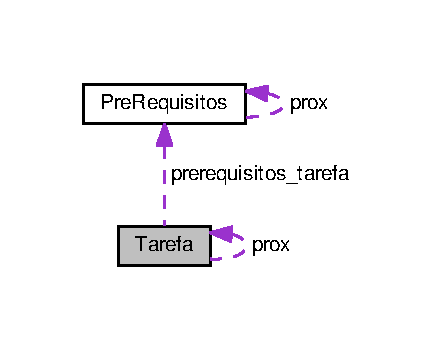
\includegraphics[width=208pt]{structTarefa__coll__graph}
\end{center}
\end{figure}
\subsection*{Atributos Públicos}
\begin{DoxyCompactItemize}
\item 
int \hyperlink{structTarefa_a1509b75b75f758e2d0502df4162366f2}{id\-\_\-tarefa}
\item 
char \hyperlink{structTarefa_a43c0db59f4e6a3031ef2a5951ad8910f}{nome\-\_\-tarefa} \mbox{[}\hyperlink{grafo_8h_a5d28dfdab86222715d699097e8cd092f}{T\-A\-M\-\_\-\-S\-T\-R\-I\-N\-G}\mbox{]}
\item 
int \hyperlink{structTarefa_a86ef331b855e3f91eec492a00171cc9c}{tarefa\-\_\-executada}
\item 
int \hyperlink{structTarefa_a7962bef326f487f4ffa7dc0f04153729}{duracao\-\_\-tarefa}
\item 
int \hyperlink{structTarefa_a7d09c30d0162c55a0aab1ad71716fae6}{inicio\-\_\-min\-\_\-tarefa}
\item 
int \hyperlink{structTarefa_a9f6369cef91f4b9d544d9e1be0bc705f}{n\-\_\-prerequisitos}
\item 
struct \hyperlink{structTarefa}{Tarefa} $\ast$ \hyperlink{structTarefa_a1b0bbf147698174596c486d12afa254e}{prox}
\item 
\hyperlink{grafo_8h_a8d260ebf15bfe9b5f9366d2245289e15}{prerequisitos} $\ast$ \hyperlink{structTarefa_abdbaac144f089e939832a4d6cbf0759a}{prerequisitos\-\_\-tarefa}
\item 
int \hyperlink{structTarefa_a4fd1b4c3fd98a3fb754116f6cc80c906}{tempo\-\_\-min}
\item 
int \hyperlink{structTarefa_a202a3c8fbee0bf74488fa057587f13df}{tempo\-\_\-inic}
\end{DoxyCompactItemize}


\subsection{Documentação dos dados membro}
\hypertarget{structTarefa_a7962bef326f487f4ffa7dc0f04153729}{\index{Tarefa@{Tarefa}!duracao\-\_\-tarefa@{duracao\-\_\-tarefa}}
\index{duracao\-\_\-tarefa@{duracao\-\_\-tarefa}!Tarefa@{Tarefa}}
\subsubsection[{duracao\-\_\-tarefa}]{\setlength{\rightskip}{0pt plus 5cm}int Tarefa\-::duracao\-\_\-tarefa}}\label{structTarefa_a7962bef326f487f4ffa7dc0f04153729}
\hypertarget{structTarefa_a1509b75b75f758e2d0502df4162366f2}{\index{Tarefa@{Tarefa}!id\-\_\-tarefa@{id\-\_\-tarefa}}
\index{id\-\_\-tarefa@{id\-\_\-tarefa}!Tarefa@{Tarefa}}
\subsubsection[{id\-\_\-tarefa}]{\setlength{\rightskip}{0pt plus 5cm}int Tarefa\-::id\-\_\-tarefa}}\label{structTarefa_a1509b75b75f758e2d0502df4162366f2}
\hypertarget{structTarefa_a7d09c30d0162c55a0aab1ad71716fae6}{\index{Tarefa@{Tarefa}!inicio\-\_\-min\-\_\-tarefa@{inicio\-\_\-min\-\_\-tarefa}}
\index{inicio\-\_\-min\-\_\-tarefa@{inicio\-\_\-min\-\_\-tarefa}!Tarefa@{Tarefa}}
\subsubsection[{inicio\-\_\-min\-\_\-tarefa}]{\setlength{\rightskip}{0pt plus 5cm}int Tarefa\-::inicio\-\_\-min\-\_\-tarefa}}\label{structTarefa_a7d09c30d0162c55a0aab1ad71716fae6}
\hypertarget{structTarefa_a9f6369cef91f4b9d544d9e1be0bc705f}{\index{Tarefa@{Tarefa}!n\-\_\-prerequisitos@{n\-\_\-prerequisitos}}
\index{n\-\_\-prerequisitos@{n\-\_\-prerequisitos}!Tarefa@{Tarefa}}
\subsubsection[{n\-\_\-prerequisitos}]{\setlength{\rightskip}{0pt plus 5cm}int Tarefa\-::n\-\_\-prerequisitos}}\label{structTarefa_a9f6369cef91f4b9d544d9e1be0bc705f}
\hypertarget{structTarefa_a43c0db59f4e6a3031ef2a5951ad8910f}{\index{Tarefa@{Tarefa}!nome\-\_\-tarefa@{nome\-\_\-tarefa}}
\index{nome\-\_\-tarefa@{nome\-\_\-tarefa}!Tarefa@{Tarefa}}
\subsubsection[{nome\-\_\-tarefa}]{\setlength{\rightskip}{0pt plus 5cm}char Tarefa\-::nome\-\_\-tarefa\mbox{[}{\bf T\-A\-M\-\_\-\-S\-T\-R\-I\-N\-G}\mbox{]}}}\label{structTarefa_a43c0db59f4e6a3031ef2a5951ad8910f}
\hypertarget{structTarefa_abdbaac144f089e939832a4d6cbf0759a}{\index{Tarefa@{Tarefa}!prerequisitos\-\_\-tarefa@{prerequisitos\-\_\-tarefa}}
\index{prerequisitos\-\_\-tarefa@{prerequisitos\-\_\-tarefa}!Tarefa@{Tarefa}}
\subsubsection[{prerequisitos\-\_\-tarefa}]{\setlength{\rightskip}{0pt plus 5cm}{\bf prerequisitos}$\ast$ Tarefa\-::prerequisitos\-\_\-tarefa}}\label{structTarefa_abdbaac144f089e939832a4d6cbf0759a}
\hypertarget{structTarefa_a1b0bbf147698174596c486d12afa254e}{\index{Tarefa@{Tarefa}!prox@{prox}}
\index{prox@{prox}!Tarefa@{Tarefa}}
\subsubsection[{prox}]{\setlength{\rightskip}{0pt plus 5cm}struct {\bf Tarefa}$\ast$ Tarefa\-::prox}}\label{structTarefa_a1b0bbf147698174596c486d12afa254e}
\hypertarget{structTarefa_a86ef331b855e3f91eec492a00171cc9c}{\index{Tarefa@{Tarefa}!tarefa\-\_\-executada@{tarefa\-\_\-executada}}
\index{tarefa\-\_\-executada@{tarefa\-\_\-executada}!Tarefa@{Tarefa}}
\subsubsection[{tarefa\-\_\-executada}]{\setlength{\rightskip}{0pt plus 5cm}int Tarefa\-::tarefa\-\_\-executada}}\label{structTarefa_a86ef331b855e3f91eec492a00171cc9c}
\hypertarget{structTarefa_a202a3c8fbee0bf74488fa057587f13df}{\index{Tarefa@{Tarefa}!tempo\-\_\-inic@{tempo\-\_\-inic}}
\index{tempo\-\_\-inic@{tempo\-\_\-inic}!Tarefa@{Tarefa}}
\subsubsection[{tempo\-\_\-inic}]{\setlength{\rightskip}{0pt plus 5cm}int Tarefa\-::tempo\-\_\-inic}}\label{structTarefa_a202a3c8fbee0bf74488fa057587f13df}
\hypertarget{structTarefa_a4fd1b4c3fd98a3fb754116f6cc80c906}{\index{Tarefa@{Tarefa}!tempo\-\_\-min@{tempo\-\_\-min}}
\index{tempo\-\_\-min@{tempo\-\_\-min}!Tarefa@{Tarefa}}
\subsubsection[{tempo\-\_\-min}]{\setlength{\rightskip}{0pt plus 5cm}int Tarefa\-::tempo\-\_\-min}}\label{structTarefa_a4fd1b4c3fd98a3fb754116f6cc80c906}


A documentação para esta estrutura foi gerada a partir do seguinte ficheiro\-:\begin{DoxyCompactItemize}
\item 
include/\hyperlink{grafo_8h}{grafo.\-h}\end{DoxyCompactItemize}

\hypertarget{structvetor}{\section{Referência à estrutura vetor}
\label{structvetor}\index{vetor@{vetor}}
}
\subsection*{Atributos Públicos}
\begin{DoxyCompactItemize}
\item 
int \hyperlink{structvetor_ab3b17d0ddfedcab54733c05868851565}{id\-\_\-tarefa}
\item 
int \hyperlink{structvetor_adff1a7b5c98b24c566ae273b5212938e}{tempo\-\_\-min}
\end{DoxyCompactItemize}


\subsection{Documentação dos dados membro}
\hypertarget{structvetor_ab3b17d0ddfedcab54733c05868851565}{\index{vetor@{vetor}!id\-\_\-tarefa@{id\-\_\-tarefa}}
\index{id\-\_\-tarefa@{id\-\_\-tarefa}!vetor@{vetor}}
\subsubsection[{id\-\_\-tarefa}]{\setlength{\rightskip}{0pt plus 5cm}int vetor\-::id\-\_\-tarefa}}\label{structvetor_ab3b17d0ddfedcab54733c05868851565}
\hypertarget{structvetor_adff1a7b5c98b24c566ae273b5212938e}{\index{vetor@{vetor}!tempo\-\_\-min@{tempo\-\_\-min}}
\index{tempo\-\_\-min@{tempo\-\_\-min}!vetor@{vetor}}
\subsubsection[{tempo\-\_\-min}]{\setlength{\rightskip}{0pt plus 5cm}int vetor\-::tempo\-\_\-min}}\label{structvetor_adff1a7b5c98b24c566ae273b5212938e}


A documentação para esta estrutura foi gerada a partir do seguinte ficheiro\-:\begin{DoxyCompactItemize}
\item 
code/\hyperlink{grafo_8cc}{grafo.\-cc}\end{DoxyCompactItemize}

\chapter{Documentação do ficheiro}
\hypertarget{grafo_8cc}{\section{Referência ao ficheiro code/grafo.cc}
\label{grafo_8cc}\index{code/grafo.\-cc@{code/grafo.\-cc}}
}
{\ttfamily \#include $<$stdio.\-h$>$}\\*
{\ttfamily \#include $<$stdlib.\-h$>$}\\*
{\ttfamily \#include $<$string.\-h$>$}\\*
{\ttfamily \#include \char`\"{}grafo.\-h\char`\"{}}\\*
\subsection*{Componentes}
\begin{DoxyCompactItemize}
\item 
struct \hyperlink{structLISTA}{L\-I\-S\-T\-A}
\item 
struct \hyperlink{structvetor}{vetor}
\end{DoxyCompactItemize}
\subsection*{Macros}
\begin{DoxyCompactItemize}
\item 
\#define \hyperlink{grafo_8cc_a9e310b9f673a2ac6b8090780f3027fbf}{M\-A\-X\-\_\-\-L\-I\-N\-H\-A}~1000
\end{DoxyCompactItemize}
\subsection*{Definições de tipos}
\begin{DoxyCompactItemize}
\item 
typedef struct \hyperlink{structLISTA}{L\-I\-S\-T\-A} \hyperlink{grafo_8cc_ae376123dbe171a2f5b6a342381f9c6b0}{lista}
\end{DoxyCompactItemize}
\subsection*{Funções}
\begin{DoxyCompactItemize}
\item 
\hyperlink{grafo_8h_abfb99265d91141543f92efaec783231d}{grafo} $\ast$ \hyperlink{grafo_8cc_aa0ebaaf04a0e9c455c6571246b5c1e15}{cria\-\_\-grafo} ()
\item 
\hyperlink{grafo_8h_abfb99265d91141543f92efaec783231d}{grafo} $\ast$ \hyperlink{grafo_8cc_a563a8912631e461ec1d9a2bff50426d9}{insere\-\_\-tarefa} (\hyperlink{grafo_8h_abfb99265d91141543f92efaec783231d}{grafo} $\ast$G, int id\-\_\-tarefa, char $\ast$nome\-\_\-tarefa, int tarefa\-\_\-executada, int duracao\-\_\-tarefa, int inicio\-\_\-min\-\_\-tarefa, int n\-\_\-prerequisitos)
\item 
\hyperlink{grafo_8h_abfb99265d91141543f92efaec783231d}{grafo} $\ast$ \hyperlink{grafo_8cc_adaeb2e2aa0bf8a2fbb149376a33bd443}{edita\-\_\-tarefa} (\hyperlink{grafo_8h_abfb99265d91141543f92efaec783231d}{grafo} $\ast$G, int id\-\_\-tarefa, int novo\-\_\-id\-\_\-tarefa, char $\ast$nome\-\_\-tarefa, int tarefa\-\_\-executada, int duracao\-\_\-tarefa, int inicio\-\_\-min\-\_\-tarefa, int n\-\_\-prerequisitos, int $\ast$id\-\_\-prerequisitos, int flag)
\item 
\hyperlink{grafo_8h_abfb99265d91141543f92efaec783231d}{grafo} $\ast$ \hyperlink{grafo_8cc_a3fe6389b74d0356a95800a3d29d7d664}{insere\-\_\-prerequisitos} (\hyperlink{grafo_8h_abfb99265d91141543f92efaec783231d}{grafo} $\ast$G, int id\-\_\-tarefa, int id\-\_\-prerequisito)
\item 
\hyperlink{grafo_8h_ab156210f10bb550f6d61bea964f08c22}{tarefa} $\ast$ \hyperlink{grafo_8cc_a0e6585acadedc05719f93fa778cf1dcb}{procura\-\_\-tarefa} (\hyperlink{grafo_8h_abfb99265d91141543f92efaec783231d}{grafo} $\ast$G, int id\-\_\-tarefa)
\item 
\hyperlink{grafo_8h_abfb99265d91141543f92efaec783231d}{grafo} $\ast$ \hyperlink{grafo_8cc_abab0a8730861a86fe9a0713b3dcc018b}{remove\-\_\-tarefa} (\hyperlink{grafo_8h_abfb99265d91141543f92efaec783231d}{grafo} $\ast$G, int id\-\_\-tarefa)
\item 
\hyperlink{grafo_8h_abfb99265d91141543f92efaec783231d}{grafo} $\ast$ \hyperlink{grafo_8cc_ad1f78512cd30c15264c68265f61296a6}{remove\-\_\-prerequisitos} (\hyperlink{grafo_8h_abfb99265d91141543f92efaec783231d}{grafo} $\ast$G, int id\-\_\-tarefa)
\item 
\hyperlink{grafo_8h_abfb99265d91141543f92efaec783231d}{grafo} $\ast$ \hyperlink{grafo_8cc_a07e2bda52af22bd5988dfab266b696f3}{le\-\_\-grafo} (F\-I\-L\-E $\ast$fp)
\item 
void \hyperlink{grafo_8cc_ac7a63f8753e7dbbb4117e6d4ebaa5933}{imprime\-\_\-grafo} (\hyperlink{grafo_8h_abfb99265d91141543f92efaec783231d}{grafo} $\ast$G, char $\ast$nome\-\_\-arq)
\item 
void \hyperlink{grafo_8cc_a64cc9fac8ef1d2aa018e1bad3e43d87e}{libera\-\_\-grafo} (\hyperlink{grafo_8h_abfb99265d91141543f92efaec783231d}{grafo} $\ast$G)
\item 
int \hyperlink{grafo_8cc_ad44b772951e7f095b7ad67dbddbc5404}{verifica\-\_\-consistencia} (\hyperlink{grafo_8h_abfb99265d91141543f92efaec783231d}{grafo} $\ast$G)
\item 
int \hyperlink{grafo_8cc_a1e996ff4a17fa0e42fc8ff6bdc605dc1}{pesquisa\-\_\-tarefa} (\hyperlink{grafo_8h_abfb99265d91141543f92efaec783231d}{grafo} $\ast$G, int id\-\_\-tarefa)
\item 
int \hyperlink{grafo_8cc_aacb0f98cd7a5b04836f1cffb745666f1}{pesquisa\-\_\-prerequisitos} (\hyperlink{grafo_8h_abfb99265d91141543f92efaec783231d}{grafo} $\ast$G, int id\-\_\-tarefa, int id\-\_\-prerequisito)
\item 
int \hyperlink{grafo_8cc_a6884bc1455bdfb3648b3e2514998e599}{tempo\-\_\-minimo} (\hyperlink{grafo_8h_abfb99265d91141543f92efaec783231d}{grafo} $\ast$G, int id\-\_\-tarefa)
\item 
\hyperlink{grafo_8cc_ae376123dbe171a2f5b6a342381f9c6b0}{lista} $\ast$ \hyperlink{grafo_8cc_acbf9093cdf86cc258309a203729436b2}{insere\-\_\-lista} (\hyperlink{grafo_8cc_ae376123dbe171a2f5b6a342381f9c6b0}{lista} $\ast$a, int id)
\item 
\hyperlink{grafo_8cc_ae376123dbe171a2f5b6a342381f9c6b0}{lista} $\ast$ \hyperlink{grafo_8cc_ae12d615ab927bce766dcc94b9f1b404d}{remove\-\_\-lista} (\hyperlink{grafo_8cc_ae376123dbe171a2f5b6a342381f9c6b0}{lista} $\ast$a, int id, int $\ast$removeu)
\item 
int \hyperlink{grafo_8cc_a57212202dfe77e7368840b67dd5fd46c}{tempo\-\_\-minimo\-\_\-total} (\hyperlink{grafo_8h_abfb99265d91141543f92efaec783231d}{grafo} $\ast$G)
\item 
int \hyperlink{grafo_8cc_a755ed9b778398a7614e61bdb3084717b}{compara} (const void $\ast$a, const void $\ast$b)
\item 
int $\ast$ \hyperlink{grafo_8cc_af11c94adb2bfc46d6f00ac0536bcddab}{caminhos} (\hyperlink{grafo_8h_abfb99265d91141543f92efaec783231d}{grafo} $\ast$G)
\item 
int $\ast$ \hyperlink{grafo_8cc_abce1552216c6841949c616cecd5a4c0b}{tarefas\-\_\-concluidas} (\hyperlink{grafo_8h_abfb99265d91141543f92efaec783231d}{grafo} $\ast$G, int periodo)
\end{DoxyCompactItemize}


\subsection{Documentação das macros}
\hypertarget{grafo_8cc_a9e310b9f673a2ac6b8090780f3027fbf}{\index{grafo.\-cc@{grafo.\-cc}!M\-A\-X\-\_\-\-L\-I\-N\-H\-A@{M\-A\-X\-\_\-\-L\-I\-N\-H\-A}}
\index{M\-A\-X\-\_\-\-L\-I\-N\-H\-A@{M\-A\-X\-\_\-\-L\-I\-N\-H\-A}!grafo.cc@{grafo.\-cc}}
\subsubsection[{M\-A\-X\-\_\-\-L\-I\-N\-H\-A}]{\setlength{\rightskip}{0pt plus 5cm}\#define M\-A\-X\-\_\-\-L\-I\-N\-H\-A~1000}}\label{grafo_8cc_a9e310b9f673a2ac6b8090780f3027fbf}


\subsection{Documentação dos tipos}
\hypertarget{grafo_8cc_ae376123dbe171a2f5b6a342381f9c6b0}{\index{grafo.\-cc@{grafo.\-cc}!lista@{lista}}
\index{lista@{lista}!grafo.cc@{grafo.\-cc}}
\subsubsection[{lista}]{\setlength{\rightskip}{0pt plus 5cm}typedef struct {\bf L\-I\-S\-T\-A}  {\bf lista}}}\label{grafo_8cc_ae376123dbe171a2f5b6a342381f9c6b0}


\subsection{Documentação das funções}
\hypertarget{grafo_8cc_af11c94adb2bfc46d6f00ac0536bcddab}{\index{grafo.\-cc@{grafo.\-cc}!caminhos@{caminhos}}
\index{caminhos@{caminhos}!grafo.cc@{grafo.\-cc}}
\subsubsection[{caminhos}]{\setlength{\rightskip}{0pt plus 5cm}int$\ast$ caminhos (
\begin{DoxyParamCaption}
\item[{{\bf grafo} $\ast$}]{G}
\end{DoxyParamCaption}
)}}\label{grafo_8cc_af11c94adb2bfc46d6f00ac0536bcddab}
Função\-: retornar \hyperlink{structGrafo}{Grafo} sem tarefas e pre requisitos.

Descrição\-:

Parâmetros\-:

Valor Retornado

Assertiva\-Entrada

Assertiva\-Saida \hypertarget{grafo_8cc_a755ed9b778398a7614e61bdb3084717b}{\index{grafo.\-cc@{grafo.\-cc}!compara@{compara}}
\index{compara@{compara}!grafo.cc@{grafo.\-cc}}
\subsubsection[{compara}]{\setlength{\rightskip}{0pt plus 5cm}int compara (
\begin{DoxyParamCaption}
\item[{const void $\ast$}]{a, }
\item[{const void $\ast$}]{b}
\end{DoxyParamCaption}
)}}\label{grafo_8cc_a755ed9b778398a7614e61bdb3084717b}
\hypertarget{grafo_8cc_aa0ebaaf04a0e9c455c6571246b5c1e15}{\index{grafo.\-cc@{grafo.\-cc}!cria\-\_\-grafo@{cria\-\_\-grafo}}
\index{cria\-\_\-grafo@{cria\-\_\-grafo}!grafo.cc@{grafo.\-cc}}
\subsubsection[{cria\-\_\-grafo}]{\setlength{\rightskip}{0pt plus 5cm}{\bf grafo}$\ast$ cria\-\_\-grafo (
\begin{DoxyParamCaption}
{}
\end{DoxyParamCaption}
)}}\label{grafo_8cc_aa0ebaaf04a0e9c455c6571246b5c1e15}
Função\-: retornar \hyperlink{structGrafo}{Grafo} sem tarefas e pre requisitos.

Descrição\-:

Parâmetros\-:

Valor Retornado

Assertiva\-Entrada

Assertiva\-Saida \hypertarget{grafo_8cc_adaeb2e2aa0bf8a2fbb149376a33bd443}{\index{grafo.\-cc@{grafo.\-cc}!edita\-\_\-tarefa@{edita\-\_\-tarefa}}
\index{edita\-\_\-tarefa@{edita\-\_\-tarefa}!grafo.cc@{grafo.\-cc}}
\subsubsection[{edita\-\_\-tarefa}]{\setlength{\rightskip}{0pt plus 5cm}{\bf grafo}$\ast$ edita\-\_\-tarefa (
\begin{DoxyParamCaption}
\item[{{\bf grafo} $\ast$}]{G, }
\item[{int}]{id\-\_\-tarefa, }
\item[{int}]{novo\-\_\-id\-\_\-tarefa, }
\item[{char $\ast$}]{nome\-\_\-tarefa, }
\item[{int}]{tarefa\-\_\-executada, }
\item[{int}]{duracao\-\_\-tarefa, }
\item[{int}]{inicio\-\_\-min\-\_\-tarefa, }
\item[{int}]{n\-\_\-prerequisitos, }
\item[{int $\ast$}]{id\-\_\-prerequisitos, }
\item[{int}]{flag}
\end{DoxyParamCaption}
)}}\label{grafo_8cc_adaeb2e2aa0bf8a2fbb149376a33bd443}
Função\-: retornar \hyperlink{structGrafo}{Grafo} sem tarefas e pre requisitos.

Descrição\-:

Parâmetros\-:

Valor Retornado

Assertiva\-Entrada

Assertiva\-Saida \hypertarget{grafo_8cc_ac7a63f8753e7dbbb4117e6d4ebaa5933}{\index{grafo.\-cc@{grafo.\-cc}!imprime\-\_\-grafo@{imprime\-\_\-grafo}}
\index{imprime\-\_\-grafo@{imprime\-\_\-grafo}!grafo.cc@{grafo.\-cc}}
\subsubsection[{imprime\-\_\-grafo}]{\setlength{\rightskip}{0pt plus 5cm}void imprime\-\_\-grafo (
\begin{DoxyParamCaption}
\item[{{\bf grafo} $\ast$}]{G, }
\item[{char $\ast$}]{nome\-\_\-arq}
\end{DoxyParamCaption}
)}}\label{grafo_8cc_ac7a63f8753e7dbbb4117e6d4ebaa5933}
Função\-: retornar \hyperlink{structGrafo}{Grafo} sem tarefas e pre requisitos.

Descrição\-:

Parâmetros\-:

Valor Retornado

Assertiva\-Entrada

Assertiva\-Saida \hypertarget{grafo_8cc_acbf9093cdf86cc258309a203729436b2}{\index{grafo.\-cc@{grafo.\-cc}!insere\-\_\-lista@{insere\-\_\-lista}}
\index{insere\-\_\-lista@{insere\-\_\-lista}!grafo.cc@{grafo.\-cc}}
\subsubsection[{insere\-\_\-lista}]{\setlength{\rightskip}{0pt plus 5cm}{\bf lista}$\ast$ insere\-\_\-lista (
\begin{DoxyParamCaption}
\item[{{\bf lista} $\ast$}]{a, }
\item[{int}]{id}
\end{DoxyParamCaption}
)}}\label{grafo_8cc_acbf9093cdf86cc258309a203729436b2}
\hypertarget{grafo_8cc_a3fe6389b74d0356a95800a3d29d7d664}{\index{grafo.\-cc@{grafo.\-cc}!insere\-\_\-prerequisitos@{insere\-\_\-prerequisitos}}
\index{insere\-\_\-prerequisitos@{insere\-\_\-prerequisitos}!grafo.cc@{grafo.\-cc}}
\subsubsection[{insere\-\_\-prerequisitos}]{\setlength{\rightskip}{0pt plus 5cm}{\bf grafo}$\ast$ insere\-\_\-prerequisitos (
\begin{DoxyParamCaption}
\item[{{\bf grafo} $\ast$}]{G, }
\item[{int}]{id\-\_\-tarefa, }
\item[{int}]{id\-\_\-prerequisito}
\end{DoxyParamCaption}
)}}\label{grafo_8cc_a3fe6389b74d0356a95800a3d29d7d664}
Função\-: retornar \hyperlink{structGrafo}{Grafo} sem tarefas e pre requisitos.

Descrição\-:

Parâmetros\-:

Valor Retornado

Assertiva\-Entrada

Assertiva\-Saida \hypertarget{grafo_8cc_a563a8912631e461ec1d9a2bff50426d9}{\index{grafo.\-cc@{grafo.\-cc}!insere\-\_\-tarefa@{insere\-\_\-tarefa}}
\index{insere\-\_\-tarefa@{insere\-\_\-tarefa}!grafo.cc@{grafo.\-cc}}
\subsubsection[{insere\-\_\-tarefa}]{\setlength{\rightskip}{0pt plus 5cm}{\bf grafo}$\ast$ insere\-\_\-tarefa (
\begin{DoxyParamCaption}
\item[{{\bf grafo} $\ast$}]{G, }
\item[{int}]{id\-\_\-tarefa, }
\item[{char $\ast$}]{nome\-\_\-tarefa, }
\item[{int}]{tarefa\-\_\-executada, }
\item[{int}]{duracao\-\_\-tarefa, }
\item[{int}]{inicio\-\_\-min\-\_\-tarefa, }
\item[{int}]{n\-\_\-prerequisitos}
\end{DoxyParamCaption}
)}}\label{grafo_8cc_a563a8912631e461ec1d9a2bff50426d9}
Função\-: retornar \hyperlink{structGrafo}{Grafo} sem tarefas e pre requisitos.

Descrição\-:

Parâmetros\-:

Valor Retornado

Assertiva\-Entrada

Assertiva\-Saida \hypertarget{grafo_8cc_a07e2bda52af22bd5988dfab266b696f3}{\index{grafo.\-cc@{grafo.\-cc}!le\-\_\-grafo@{le\-\_\-grafo}}
\index{le\-\_\-grafo@{le\-\_\-grafo}!grafo.cc@{grafo.\-cc}}
\subsubsection[{le\-\_\-grafo}]{\setlength{\rightskip}{0pt plus 5cm}{\bf grafo}$\ast$ le\-\_\-grafo (
\begin{DoxyParamCaption}
\item[{F\-I\-L\-E $\ast$}]{fp}
\end{DoxyParamCaption}
)}}\label{grafo_8cc_a07e2bda52af22bd5988dfab266b696f3}
Função\-: retornar \hyperlink{structGrafo}{Grafo} sem tarefas e pre requisitos.

Descrição\-:

Parâmetros\-:

Valor Retornado

Assertiva\-Entrada

Assertiva\-Saida \hypertarget{grafo_8cc_a64cc9fac8ef1d2aa018e1bad3e43d87e}{\index{grafo.\-cc@{grafo.\-cc}!libera\-\_\-grafo@{libera\-\_\-grafo}}
\index{libera\-\_\-grafo@{libera\-\_\-grafo}!grafo.cc@{grafo.\-cc}}
\subsubsection[{libera\-\_\-grafo}]{\setlength{\rightskip}{0pt plus 5cm}void libera\-\_\-grafo (
\begin{DoxyParamCaption}
\item[{{\bf grafo} $\ast$}]{G}
\end{DoxyParamCaption}
)}}\label{grafo_8cc_a64cc9fac8ef1d2aa018e1bad3e43d87e}
Função\-: retornar \hyperlink{structGrafo}{Grafo} sem tarefas e pre requisitos.

Descrição\-:

Parâmetros\-:

Valor Retornado

Assertiva\-Entrada

Assertiva\-Saida \hypertarget{grafo_8cc_aacb0f98cd7a5b04836f1cffb745666f1}{\index{grafo.\-cc@{grafo.\-cc}!pesquisa\-\_\-prerequisitos@{pesquisa\-\_\-prerequisitos}}
\index{pesquisa\-\_\-prerequisitos@{pesquisa\-\_\-prerequisitos}!grafo.cc@{grafo.\-cc}}
\subsubsection[{pesquisa\-\_\-prerequisitos}]{\setlength{\rightskip}{0pt plus 5cm}int pesquisa\-\_\-prerequisitos (
\begin{DoxyParamCaption}
\item[{{\bf grafo} $\ast$}]{G, }
\item[{int}]{id\-\_\-tarefa, }
\item[{int}]{id\-\_\-prerequisito}
\end{DoxyParamCaption}
)}}\label{grafo_8cc_aacb0f98cd7a5b04836f1cffb745666f1}
Função\-: retornar \hyperlink{structGrafo}{Grafo} sem tarefas e pre requisitos.

Descrição\-:

Parâmetros\-:

Valor Retornado

Assertiva\-Entrada

Assertiva\-Saida \hypertarget{grafo_8cc_a1e996ff4a17fa0e42fc8ff6bdc605dc1}{\index{grafo.\-cc@{grafo.\-cc}!pesquisa\-\_\-tarefa@{pesquisa\-\_\-tarefa}}
\index{pesquisa\-\_\-tarefa@{pesquisa\-\_\-tarefa}!grafo.cc@{grafo.\-cc}}
\subsubsection[{pesquisa\-\_\-tarefa}]{\setlength{\rightskip}{0pt plus 5cm}int pesquisa\-\_\-tarefa (
\begin{DoxyParamCaption}
\item[{{\bf grafo} $\ast$}]{G, }
\item[{int}]{id\-\_\-tarefa}
\end{DoxyParamCaption}
)}}\label{grafo_8cc_a1e996ff4a17fa0e42fc8ff6bdc605dc1}
Função\-: retornar \hyperlink{structGrafo}{Grafo} sem tarefas e pre requisitos.

Descrição\-:

Parâmetros\-:

Valor Retornado

Assertiva\-Entrada

Assertiva\-Saida \hypertarget{grafo_8cc_a0e6585acadedc05719f93fa778cf1dcb}{\index{grafo.\-cc@{grafo.\-cc}!procura\-\_\-tarefa@{procura\-\_\-tarefa}}
\index{procura\-\_\-tarefa@{procura\-\_\-tarefa}!grafo.cc@{grafo.\-cc}}
\subsubsection[{procura\-\_\-tarefa}]{\setlength{\rightskip}{0pt plus 5cm}{\bf tarefa}$\ast$ procura\-\_\-tarefa (
\begin{DoxyParamCaption}
\item[{{\bf grafo} $\ast$}]{G, }
\item[{int}]{id\-\_\-tarefa}
\end{DoxyParamCaption}
)}}\label{grafo_8cc_a0e6585acadedc05719f93fa778cf1dcb}
Função\-: retornar \hyperlink{structGrafo}{Grafo} sem tarefas e pre requisitos.

Descrição\-:

Parâmetros\-:

Valor Retornado

Assertiva\-Entrada

Assertiva\-Saida \hypertarget{grafo_8cc_ae12d615ab927bce766dcc94b9f1b404d}{\index{grafo.\-cc@{grafo.\-cc}!remove\-\_\-lista@{remove\-\_\-lista}}
\index{remove\-\_\-lista@{remove\-\_\-lista}!grafo.cc@{grafo.\-cc}}
\subsubsection[{remove\-\_\-lista}]{\setlength{\rightskip}{0pt plus 5cm}{\bf lista}$\ast$ remove\-\_\-lista (
\begin{DoxyParamCaption}
\item[{{\bf lista} $\ast$}]{a, }
\item[{int}]{id, }
\item[{int $\ast$}]{removeu}
\end{DoxyParamCaption}
)}}\label{grafo_8cc_ae12d615ab927bce766dcc94b9f1b404d}
\hypertarget{grafo_8cc_ad1f78512cd30c15264c68265f61296a6}{\index{grafo.\-cc@{grafo.\-cc}!remove\-\_\-prerequisitos@{remove\-\_\-prerequisitos}}
\index{remove\-\_\-prerequisitos@{remove\-\_\-prerequisitos}!grafo.cc@{grafo.\-cc}}
\subsubsection[{remove\-\_\-prerequisitos}]{\setlength{\rightskip}{0pt plus 5cm}{\bf grafo}$\ast$ remove\-\_\-prerequisitos (
\begin{DoxyParamCaption}
\item[{{\bf grafo} $\ast$}]{G, }
\item[{int}]{id\-\_\-tarefa}
\end{DoxyParamCaption}
)}}\label{grafo_8cc_ad1f78512cd30c15264c68265f61296a6}
Função\-: retornar \hyperlink{structGrafo}{Grafo} sem tarefas e pre requisitos.

Descrição\-:

Parâmetros\-:

Valor Retornado

Assertiva\-Entrada

Assertiva\-Saida \hypertarget{grafo_8cc_abab0a8730861a86fe9a0713b3dcc018b}{\index{grafo.\-cc@{grafo.\-cc}!remove\-\_\-tarefa@{remove\-\_\-tarefa}}
\index{remove\-\_\-tarefa@{remove\-\_\-tarefa}!grafo.cc@{grafo.\-cc}}
\subsubsection[{remove\-\_\-tarefa}]{\setlength{\rightskip}{0pt plus 5cm}{\bf grafo}$\ast$ remove\-\_\-tarefa (
\begin{DoxyParamCaption}
\item[{{\bf grafo} $\ast$}]{G, }
\item[{int}]{id\-\_\-tarefa}
\end{DoxyParamCaption}
)}}\label{grafo_8cc_abab0a8730861a86fe9a0713b3dcc018b}
Função\-: retornar \hyperlink{structGrafo}{Grafo} sem tarefas e pre requisitos.

Descrição\-:

Parâmetros\-:

Valor Retornado

Assertiva\-Entrada

Assertiva\-Saida \hypertarget{grafo_8cc_abce1552216c6841949c616cecd5a4c0b}{\index{grafo.\-cc@{grafo.\-cc}!tarefas\-\_\-concluidas@{tarefas\-\_\-concluidas}}
\index{tarefas\-\_\-concluidas@{tarefas\-\_\-concluidas}!grafo.cc@{grafo.\-cc}}
\subsubsection[{tarefas\-\_\-concluidas}]{\setlength{\rightskip}{0pt plus 5cm}int$\ast$ tarefas\-\_\-concluidas (
\begin{DoxyParamCaption}
\item[{{\bf grafo} $\ast$}]{G, }
\item[{int}]{periodo}
\end{DoxyParamCaption}
)}}\label{grafo_8cc_abce1552216c6841949c616cecd5a4c0b}
Função\-: retornar \hyperlink{structGrafo}{Grafo} sem tarefas e pre requisitos.

Descrição\-:

Parâmetros\-:

Valor Retornado

Assertiva\-Entrada

Assertiva\-Saida \hypertarget{grafo_8cc_a6884bc1455bdfb3648b3e2514998e599}{\index{grafo.\-cc@{grafo.\-cc}!tempo\-\_\-minimo@{tempo\-\_\-minimo}}
\index{tempo\-\_\-minimo@{tempo\-\_\-minimo}!grafo.cc@{grafo.\-cc}}
\subsubsection[{tempo\-\_\-minimo}]{\setlength{\rightskip}{0pt plus 5cm}int tempo\-\_\-minimo (
\begin{DoxyParamCaption}
\item[{{\bf grafo} $\ast$}]{G, }
\item[{int}]{id\-\_\-tarefa}
\end{DoxyParamCaption}
)}}\label{grafo_8cc_a6884bc1455bdfb3648b3e2514998e599}
Função\-: retornar \hyperlink{structGrafo}{Grafo} sem tarefas e pre requisitos.

Descrição\-:

Parâmetros\-:

Valor Retornado

Assertiva\-Entrada

Assertiva\-Saida \hypertarget{grafo_8cc_a57212202dfe77e7368840b67dd5fd46c}{\index{grafo.\-cc@{grafo.\-cc}!tempo\-\_\-minimo\-\_\-total@{tempo\-\_\-minimo\-\_\-total}}
\index{tempo\-\_\-minimo\-\_\-total@{tempo\-\_\-minimo\-\_\-total}!grafo.cc@{grafo.\-cc}}
\subsubsection[{tempo\-\_\-minimo\-\_\-total}]{\setlength{\rightskip}{0pt plus 5cm}int tempo\-\_\-minimo\-\_\-total (
\begin{DoxyParamCaption}
\item[{{\bf grafo} $\ast$}]{G}
\end{DoxyParamCaption}
)}}\label{grafo_8cc_a57212202dfe77e7368840b67dd5fd46c}
Função\-: retornar \hyperlink{structGrafo}{Grafo} sem tarefas e pre requisitos.

Descrição\-:

Parâmetros\-:

Valor Retornado

Assertiva\-Entrada

Assertiva\-Saida \hypertarget{grafo_8cc_ad44b772951e7f095b7ad67dbddbc5404}{\index{grafo.\-cc@{grafo.\-cc}!verifica\-\_\-consistencia@{verifica\-\_\-consistencia}}
\index{verifica\-\_\-consistencia@{verifica\-\_\-consistencia}!grafo.cc@{grafo.\-cc}}
\subsubsection[{verifica\-\_\-consistencia}]{\setlength{\rightskip}{0pt plus 5cm}int verifica\-\_\-consistencia (
\begin{DoxyParamCaption}
\item[{{\bf grafo} $\ast$}]{G}
\end{DoxyParamCaption}
)}}\label{grafo_8cc_ad44b772951e7f095b7ad67dbddbc5404}
Função\-: retornar \hyperlink{structGrafo}{Grafo} sem tarefas e pre requisitos.

Descrição\-:

Parâmetros\-:

Valor Retornado

Assertiva\-Entrada

Assertiva\-Saida 
\hypertarget{gtest__grafo_8cc}{\section{Referência ao ficheiro code/gtest\-\_\-grafo.cc}
\label{gtest__grafo_8cc}\index{code/gtest\-\_\-grafo.\-cc@{code/gtest\-\_\-grafo.\-cc}}
}
{\ttfamily \#include \char`\"{}gtest/gtest.\-h\char`\"{}}\\*
{\ttfamily \#include \char`\"{}grafo.\-h\char`\"{}}\\*
Diagrama de dependências de inclusão para gtest\-\_\-grafo.\-cc\-:\nopagebreak
\begin{figure}[H]
\begin{center}
\leavevmode
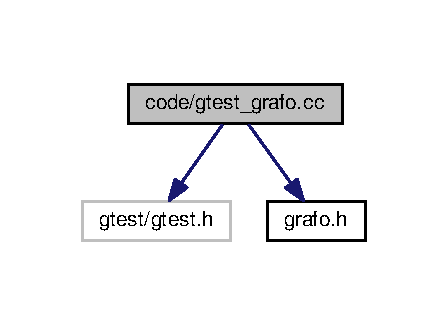
\includegraphics[width=215pt]{gtest__grafo_8cc__incl}
\end{center}
\end{figure}
\subsection*{Funções}
\begin{DoxyCompactItemize}
\item 
\hyperlink{gtest__grafo_8cc_acdd61f8b660ae6979528c7e3da0e134d}{T\-E\-S\-T} (Test\-Importa\-Tarefas\-Arquivo, \hyperlink{include_2grafo_8h_a07e2bda52af22bd5988dfab266b696f3}{le\-\_\-grafo})
\item 
\hyperlink{gtest__grafo_8cc_a207d91b43a907a510504a2f7d4c3ae7d}{T\-E\-S\-T} (Test\-Grava\-Tarefas\-Arquivo, \hyperlink{include_2grafo_8h_ac7a63f8753e7dbbb4117e6d4ebaa5933}{imprime\-\_\-grafo})
\item 
int \hyperlink{gtest__grafo_8cc_a3c04138a5bfe5d72780bb7e82a18e627}{main} (int argc, char $\ast$$\ast$argv)
\end{DoxyCompactItemize}


\subsection{Documentação das funções}
\hypertarget{gtest__grafo_8cc_a3c04138a5bfe5d72780bb7e82a18e627}{\index{gtest\-\_\-grafo.\-cc@{gtest\-\_\-grafo.\-cc}!main@{main}}
\index{main@{main}!gtest_grafo.cc@{gtest\-\_\-grafo.\-cc}}
\subsubsection[{main}]{\setlength{\rightskip}{0pt plus 5cm}int main (
\begin{DoxyParamCaption}
\item[{int}]{argc, }
\item[{char $\ast$$\ast$}]{argv}
\end{DoxyParamCaption}
)}}\label{gtest__grafo_8cc_a3c04138a5bfe5d72780bb7e82a18e627}
\hypertarget{gtest__grafo_8cc_acdd61f8b660ae6979528c7e3da0e134d}{\index{gtest\-\_\-grafo.\-cc@{gtest\-\_\-grafo.\-cc}!T\-E\-S\-T@{T\-E\-S\-T}}
\index{T\-E\-S\-T@{T\-E\-S\-T}!gtest_grafo.cc@{gtest\-\_\-grafo.\-cc}}
\subsubsection[{T\-E\-S\-T}]{\setlength{\rightskip}{0pt plus 5cm}T\-E\-S\-T (
\begin{DoxyParamCaption}
\item[{Test\-Importa\-Tarefas\-Arquivo}]{, }
\item[{{\bf le\-\_\-grafo}}]{}
\end{DoxyParamCaption}
)}}\label{gtest__grafo_8cc_acdd61f8b660ae6979528c7e3da0e134d}


Grafo de chamadas desta função\-:\nopagebreak
\begin{figure}[H]
\begin{center}
\leavevmode
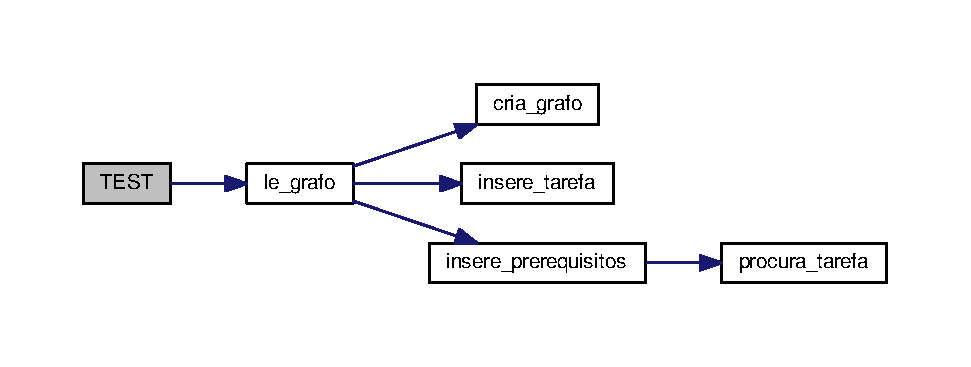
\includegraphics[width=350pt]{gtest__grafo_8cc_acdd61f8b660ae6979528c7e3da0e134d_cgraph}
\end{center}
\end{figure}


\hypertarget{gtest__grafo_8cc_a207d91b43a907a510504a2f7d4c3ae7d}{\index{gtest\-\_\-grafo.\-cc@{gtest\-\_\-grafo.\-cc}!T\-E\-S\-T@{T\-E\-S\-T}}
\index{T\-E\-S\-T@{T\-E\-S\-T}!gtest_grafo.cc@{gtest\-\_\-grafo.\-cc}}
\subsubsection[{T\-E\-S\-T}]{\setlength{\rightskip}{0pt plus 5cm}T\-E\-S\-T (
\begin{DoxyParamCaption}
\item[{Test\-Grava\-Tarefas\-Arquivo}]{, }
\item[{{\bf imprime\-\_\-grafo}}]{}
\end{DoxyParamCaption}
)}}\label{gtest__grafo_8cc_a207d91b43a907a510504a2f7d4c3ae7d}


Grafo de chamadas desta função\-:\nopagebreak
\begin{figure}[H]
\begin{center}
\leavevmode
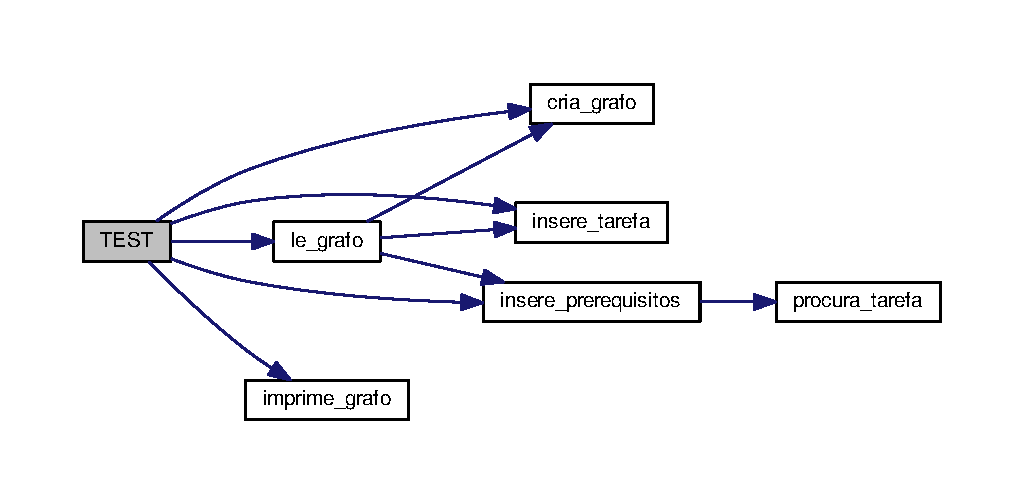
\includegraphics[width=350pt]{gtest__grafo_8cc_a207d91b43a907a510504a2f7d4c3ae7d_cgraph}
\end{center}
\end{figure}



\hypertarget{main_8cc}{\section{Referência ao ficheiro code/main.cc}
\label{main_8cc}\index{code/main.\-cc@{code/main.\-cc}}
}
{\ttfamily \#include $<$ncurses.\-h$>$}\\*
{\ttfamily \#include $<$stdlib.\-h$>$}\\*
{\ttfamily \#include $<$stdio.\-h$>$}\\*
{\ttfamily \#include $<$string.\-h$>$}\\*
{\ttfamily \#include \char`\"{}grafo.\-h\char`\"{}}\\*
Diagrama de dependências de inclusão para main.\-cc\-:\nopagebreak
\begin{figure}[H]
\begin{center}
\leavevmode
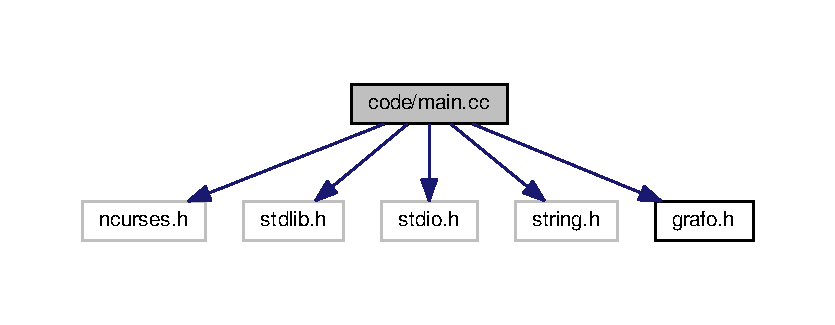
\includegraphics[width=350pt]{main_8cc__incl}
\end{center}
\end{figure}
\subsection*{Macros}
\begin{DoxyCompactItemize}
\item 
\#define \hyperlink{main_8cc_a39993a19ea179e022fb3346fdc794808}{L\-A\-R\-G\-U\-R\-A}~50
\item 
\#define \hyperlink{main_8cc_a0ca6912086aeaf9fbab770dcb97ea5c8}{A\-L\-T\-U\-R\-A}~10
\end{DoxyCompactItemize}
\subsection*{Funções}
\begin{DoxyCompactItemize}
\item 
void \hyperlink{main_8cc_a810164b29b6ded682dff19d56ec8e4b0}{print\-\_\-menu} (W\-I\-N\-D\-O\-W $\ast$menu\-\_\-win, int highlight)
\item 
void \hyperlink{main_8cc_a8b39b6c1f4d3623c384e80826e5b633e}{print\-\_\-operacoes} (W\-I\-N\-D\-O\-W $\ast$menu\-\_\-win, int highlight)
\item 
void \hyperlink{main_8cc_a4611d53166aabe6d0fb24bcfd407bd53}{print\-\_\-visualizador} (W\-I\-N\-D\-O\-W $\ast$menu\-\_\-win, int highlight)
\item 
void \hyperlink{main_8cc_ad2a06ffdf1033b3b1c11f337fa12553b}{imprimir\-Rotulo} (W\-I\-N\-D\-O\-W $\ast$tmp\-Janela, int y, int x, char $\ast$s\-Rotulo)
\item 
void \hyperlink{main_8cc_abe7109d6b800c7cd9f5c2097bc8df894}{destruir\-\_\-menu} (W\-I\-N\-D\-O\-W $\ast$menu\-\_\-win)
\item 
char $\ast$ \hyperlink{main_8cc_af680447ac3023912e86df70f144373d8}{importar\-\_\-de\-\_\-arquivo} (char $\ast$nome\-Arquivo)
\item 
void \hyperlink{main_8cc_aef0e5ebaf10f94ec3baf710468b2bca8}{erro\-\_\-insere\-\_\-pre\-\_\-requisito} ()
\item 
void \hyperlink{main_8cc_acec6efd5f1ee225764d814040f142268}{erro\-\_\-id\-\_\-existente} ()
\item 
void \hyperlink{main_8cc_acf899fb4107a26f962c26ec5292148cd}{erro\-\_\-id\-\_\-invalido} ()
\item 
void \hyperlink{main_8cc_a8e3083a90f6cf70bdfd6abd70494c74e}{erro\-\_\-id\-\_\-inexistente} ()
\item 
\hyperlink{code_2grafo_8h_abfb99265d91141543f92efaec783231d}{grafo} $\ast$ \hyperlink{main_8cc_a16c89e840263b1af21caf3211b6640b2}{inserir\-\_\-novo\-\_\-pre\-\_\-requisito} (\hyperlink{code_2grafo_8h_abfb99265d91141543f92efaec783231d}{grafo} $\ast$G)
\item 
int \hyperlink{main_8cc_a5f90fb7a7aa9c2393d70b4f95d675955}{tela\-\_\-inserir\-\_\-pre\-\_\-requisito\-\_\-edicao} ()
\item 
\hyperlink{code_2grafo_8h_abfb99265d91141543f92efaec783231d}{grafo} $\ast$ \hyperlink{main_8cc_a5c0ceb9634231b92e0dfc9db33b727fa}{tela\-\_\-inserir\-\_\-pre\-\_\-requisito} (\hyperlink{code_2grafo_8h_abfb99265d91141543f92efaec783231d}{grafo} $\ast$G, int n\-\_\-prerequisitos, int id\-\_\-tarefa)
\item 
\hyperlink{code_2grafo_8h_abfb99265d91141543f92efaec783231d}{grafo} $\ast$ \hyperlink{main_8cc_adb3b0c3b009c68f86673eb7bdeef601c}{inserir\-\_\-tarefa} (\hyperlink{code_2grafo_8h_abfb99265d91141543f92efaec783231d}{grafo} $\ast$G)
\item 
void \hyperlink{main_8cc_abc30d77428eefe83c569f49b7e48a7f8}{imprimir\-\_\-em\-\_\-arquivo} (\hyperlink{code_2grafo_8h_abfb99265d91141543f92efaec783231d}{grafo} $\ast$G)
\item 
\hyperlink{code_2grafo_8h_abfb99265d91141543f92efaec783231d}{grafo} $\ast$ \hyperlink{main_8cc_a8d8002aa0f76981dad9ce30329767981}{edicao\-\_\-tarefa} (\hyperlink{code_2grafo_8h_abfb99265d91141543f92efaec783231d}{grafo} $\ast$G, int id)
\item 
\hyperlink{code_2grafo_8h_abfb99265d91141543f92efaec783231d}{grafo} $\ast$ \hyperlink{main_8cc_a7769e05575359d89d7467b1e46940ecf}{editar\-\_\-tarefa} (\hyperlink{code_2grafo_8h_abfb99265d91141543f92efaec783231d}{grafo} $\ast$G)
\item 
\hyperlink{code_2grafo_8h_abfb99265d91141543f92efaec783231d}{grafo} $\ast$ \hyperlink{main_8cc_ab5f698491708904442d9d4f8583cd809}{remover\-\_\-tarefa} (\hyperlink{code_2grafo_8h_abfb99265d91141543f92efaec783231d}{grafo} $\ast$G)
\item 
void \hyperlink{main_8cc_aa0ac4a2d1125c89ec5acc37dfde748c6}{ver\-\_\-tarefas} (\hyperlink{code_2grafo_8h_abfb99265d91141543f92efaec783231d}{grafo} $\ast$G)
\item 
void \hyperlink{main_8cc_a4f8f29b1eba21e0b51992f8de173a582}{mostrar\-\_\-pre\-\_\-requisitos} (\hyperlink{code_2grafo_8h_abfb99265d91141543f92efaec783231d}{grafo} $\ast$G)
\item 
void \hyperlink{main_8cc_ab05b93d97a47c67aab51426cdad29a86}{ver\-\_\-tarefas\-\_\-concluidas} (\hyperlink{code_2grafo_8h_abfb99265d91141543f92efaec783231d}{grafo} $\ast$G)
\item 
\hyperlink{code_2grafo_8h_abfb99265d91141543f92efaec783231d}{grafo} $\ast$ \hyperlink{main_8cc_ae96b9adf5e390d1a516e3fe5164714cc}{remover\-\_\-pre\-\_\-requisitos} (\hyperlink{code_2grafo_8h_abfb99265d91141543f92efaec783231d}{grafo} $\ast$G)
\item 
void \hyperlink{main_8cc_aaaa25a5b0eda0fab944a03026249b324}{mostrar\-\_\-tarefas\-\_\-filtradas} (\hyperlink{code_2grafo_8h_abfb99265d91141543f92efaec783231d}{grafo} $\ast$G, int $\ast$tarefas)
\item 
void \hyperlink{main_8cc_adcc550070c8292efdd63f7df8bbdd58a}{filtrar\-\_\-tarefas\-\_\-completadas} (\hyperlink{code_2grafo_8h_abfb99265d91141543f92efaec783231d}{grafo} $\ast$G)
\item 
void \hyperlink{main_8cc_a5d247f6e8ee275a8cd007f922ae2acb3}{visualizador\-\_\-tarefas} (\hyperlink{code_2grafo_8h_abfb99265d91141543f92efaec783231d}{grafo} $\ast$G)
\item 
\hyperlink{code_2grafo_8h_abfb99265d91141543f92efaec783231d}{grafo} $\ast$ \hyperlink{main_8cc_af852bc15cf3d5217386a9bb0bf3b9abd}{operacoes\-\_\-grafo} (\hyperlink{code_2grafo_8h_abfb99265d91141543f92efaec783231d}{grafo} $\ast$G)
\item 
\hyperlink{code_2grafo_8h_abfb99265d91141543f92efaec783231d}{grafo} $\ast$ \hyperlink{main_8cc_af1ccf694bcf905341f10b534e5a272fa}{abrir\-\_\-arquivo} (char $\ast$nome\-Arquivo)
\item 
int \hyperlink{main_8cc_ae66f6b31b5ad750f1fe042a706a4e3d4}{main} ()
\end{DoxyCompactItemize}
\subsection*{Variáveis}
\begin{DoxyCompactItemize}
\item 
int \hyperlink{main_8cc_a8f0744c55ee97ebf34757f8499a66139}{startx} = 0
\item 
int \hyperlink{main_8cc_a19e264821cbd530471c1cf985d7cd239}{starty} = 0
\item 
char \hyperlink{main_8cc_a7e3eb983c89b73fc26206eb49d9e53f6}{v\-Opcoes} \mbox{[}3\mbox{]}\mbox{[}70\mbox{]}
\item 
char \hyperlink{main_8cc_a282382d81ff49bb355edf4b0e0c33ab5}{v\-Operacoes} \mbox{[}8\mbox{]}\mbox{[}70\mbox{]}
\item 
char \hyperlink{main_8cc_ac830448011ecd7178e23030edbff0311}{v\-Visualizador} \mbox{[}6\mbox{]}\mbox{[}70\mbox{]}
\item 
int \hyperlink{main_8cc_a24167c503992e21d9d3b767742346d4b}{n\-\_\-opcoes} = 3
\item 
int \hyperlink{main_8cc_a4e96567620b8107a3844f6a3b5860c74}{n\-\_\-operacoes} = 8
\item 
int \hyperlink{main_8cc_a44042648455eb7c48a35466047cd5911}{n\-\_\-visualizador} = 6
\end{DoxyCompactItemize}


\subsection{Documentação das macros}
\hypertarget{main_8cc_a0ca6912086aeaf9fbab770dcb97ea5c8}{\index{main.\-cc@{main.\-cc}!A\-L\-T\-U\-R\-A@{A\-L\-T\-U\-R\-A}}
\index{A\-L\-T\-U\-R\-A@{A\-L\-T\-U\-R\-A}!main.cc@{main.\-cc}}
\subsubsection[{A\-L\-T\-U\-R\-A}]{\setlength{\rightskip}{0pt plus 5cm}\#define A\-L\-T\-U\-R\-A~10}}\label{main_8cc_a0ca6912086aeaf9fbab770dcb97ea5c8}
\hypertarget{main_8cc_a39993a19ea179e022fb3346fdc794808}{\index{main.\-cc@{main.\-cc}!L\-A\-R\-G\-U\-R\-A@{L\-A\-R\-G\-U\-R\-A}}
\index{L\-A\-R\-G\-U\-R\-A@{L\-A\-R\-G\-U\-R\-A}!main.cc@{main.\-cc}}
\subsubsection[{L\-A\-R\-G\-U\-R\-A}]{\setlength{\rightskip}{0pt plus 5cm}\#define L\-A\-R\-G\-U\-R\-A~50}}\label{main_8cc_a39993a19ea179e022fb3346fdc794808}


\subsection{Documentação das funções}
\hypertarget{main_8cc_af1ccf694bcf905341f10b534e5a272fa}{\index{main.\-cc@{main.\-cc}!abrir\-\_\-arquivo@{abrir\-\_\-arquivo}}
\index{abrir\-\_\-arquivo@{abrir\-\_\-arquivo}!main.cc@{main.\-cc}}
\subsubsection[{abrir\-\_\-arquivo}]{\setlength{\rightskip}{0pt plus 5cm}{\bf grafo}$\ast$ abrir\-\_\-arquivo (
\begin{DoxyParamCaption}
\item[{char $\ast$}]{nome\-Arquivo}
\end{DoxyParamCaption}
)}}\label{main_8cc_af1ccf694bcf905341f10b534e5a272fa}


Grafo de chamadas desta função\-:\nopagebreak
\begin{figure}[H]
\begin{center}
\leavevmode
\includegraphics[height=550pt]{main_8cc_af1ccf694bcf905341f10b534e5a272fa_cgraph}
\end{center}
\end{figure}




Este é o diagrama das funções que utilizam esta função\-:\nopagebreak
\begin{figure}[H]
\begin{center}
\leavevmode
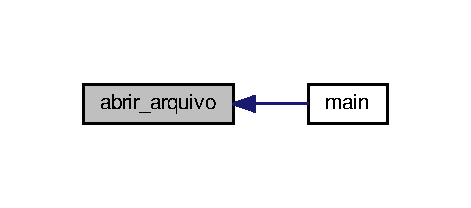
\includegraphics[width=226pt]{main_8cc_af1ccf694bcf905341f10b534e5a272fa_icgraph}
\end{center}
\end{figure}


\hypertarget{main_8cc_abe7109d6b800c7cd9f5c2097bc8df894}{\index{main.\-cc@{main.\-cc}!destruir\-\_\-menu@{destruir\-\_\-menu}}
\index{destruir\-\_\-menu@{destruir\-\_\-menu}!main.cc@{main.\-cc}}
\subsubsection[{destruir\-\_\-menu}]{\setlength{\rightskip}{0pt plus 5cm}void destruir\-\_\-menu (
\begin{DoxyParamCaption}
\item[{W\-I\-N\-D\-O\-W $\ast$}]{menu\-\_\-win}
\end{DoxyParamCaption}
)}}\label{main_8cc_abe7109d6b800c7cd9f5c2097bc8df894}


Este é o diagrama das funções que utilizam esta função\-:\nopagebreak
\begin{figure}[H]
\begin{center}
\leavevmode
\includegraphics[width=350pt]{main_8cc_abe7109d6b800c7cd9f5c2097bc8df894_icgraph}
\end{center}
\end{figure}


\hypertarget{main_8cc_a8d8002aa0f76981dad9ce30329767981}{\index{main.\-cc@{main.\-cc}!edicao\-\_\-tarefa@{edicao\-\_\-tarefa}}
\index{edicao\-\_\-tarefa@{edicao\-\_\-tarefa}!main.cc@{main.\-cc}}
\subsubsection[{edicao\-\_\-tarefa}]{\setlength{\rightskip}{0pt plus 5cm}{\bf grafo}$\ast$ edicao\-\_\-tarefa (
\begin{DoxyParamCaption}
\item[{{\bf grafo} $\ast$}]{G, }
\item[{int}]{id}
\end{DoxyParamCaption}
)}}\label{main_8cc_a8d8002aa0f76981dad9ce30329767981}


Grafo de chamadas desta função\-:\nopagebreak
\begin{figure}[H]
\begin{center}
\leavevmode
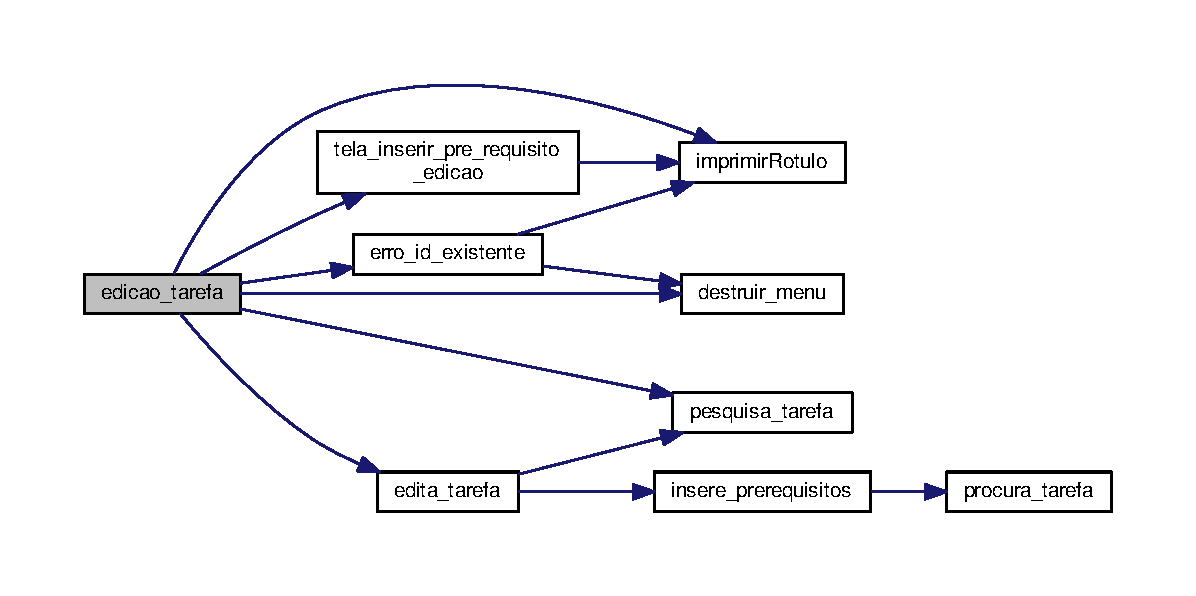
\includegraphics[width=350pt]{main_8cc_a8d8002aa0f76981dad9ce30329767981_cgraph}
\end{center}
\end{figure}




Este é o diagrama das funções que utilizam esta função\-:\nopagebreak
\begin{figure}[H]
\begin{center}
\leavevmode
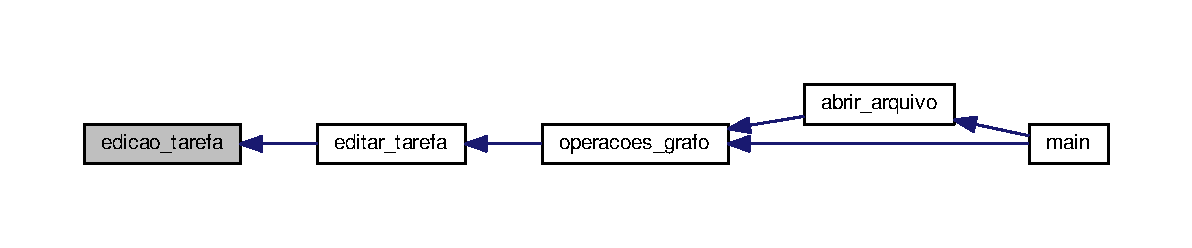
\includegraphics[width=350pt]{main_8cc_a8d8002aa0f76981dad9ce30329767981_icgraph}
\end{center}
\end{figure}


\hypertarget{main_8cc_a7769e05575359d89d7467b1e46940ecf}{\index{main.\-cc@{main.\-cc}!editar\-\_\-tarefa@{editar\-\_\-tarefa}}
\index{editar\-\_\-tarefa@{editar\-\_\-tarefa}!main.cc@{main.\-cc}}
\subsubsection[{editar\-\_\-tarefa}]{\setlength{\rightskip}{0pt plus 5cm}{\bf grafo}$\ast$ editar\-\_\-tarefa (
\begin{DoxyParamCaption}
\item[{{\bf grafo} $\ast$}]{G}
\end{DoxyParamCaption}
)}}\label{main_8cc_a7769e05575359d89d7467b1e46940ecf}


Grafo de chamadas desta função\-:\nopagebreak
\begin{figure}[H]
\begin{center}
\leavevmode
\includegraphics[width=350pt]{main_8cc_a7769e05575359d89d7467b1e46940ecf_cgraph}
\end{center}
\end{figure}




Este é o diagrama das funções que utilizam esta função\-:\nopagebreak
\begin{figure}[H]
\begin{center}
\leavevmode
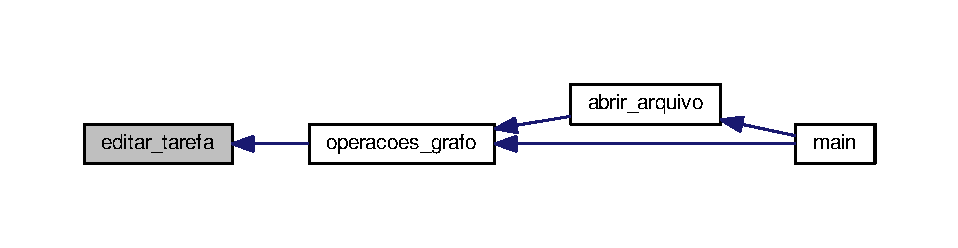
\includegraphics[width=350pt]{main_8cc_a7769e05575359d89d7467b1e46940ecf_icgraph}
\end{center}
\end{figure}


\hypertarget{main_8cc_acec6efd5f1ee225764d814040f142268}{\index{main.\-cc@{main.\-cc}!erro\-\_\-id\-\_\-existente@{erro\-\_\-id\-\_\-existente}}
\index{erro\-\_\-id\-\_\-existente@{erro\-\_\-id\-\_\-existente}!main.cc@{main.\-cc}}
\subsubsection[{erro\-\_\-id\-\_\-existente}]{\setlength{\rightskip}{0pt plus 5cm}void erro\-\_\-id\-\_\-existente (
\begin{DoxyParamCaption}
{}
\end{DoxyParamCaption}
)}}\label{main_8cc_acec6efd5f1ee225764d814040f142268}


Grafo de chamadas desta função\-:\nopagebreak
\begin{figure}[H]
\begin{center}
\leavevmode
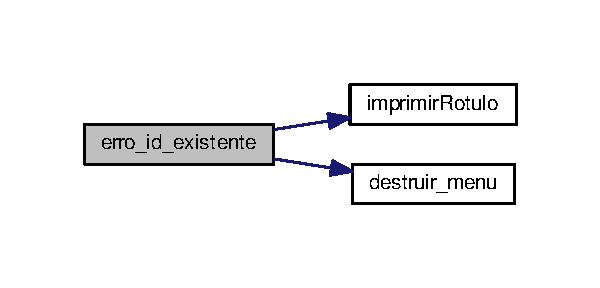
\includegraphics[width=288pt]{main_8cc_acec6efd5f1ee225764d814040f142268_cgraph}
\end{center}
\end{figure}




Este é o diagrama das funções que utilizam esta função\-:\nopagebreak
\begin{figure}[H]
\begin{center}
\leavevmode
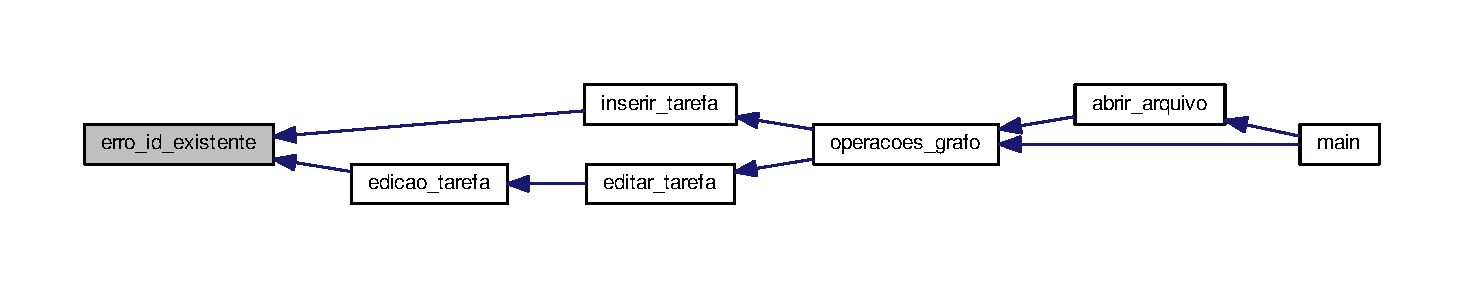
\includegraphics[width=350pt]{main_8cc_acec6efd5f1ee225764d814040f142268_icgraph}
\end{center}
\end{figure}


\hypertarget{main_8cc_a8e3083a90f6cf70bdfd6abd70494c74e}{\index{main.\-cc@{main.\-cc}!erro\-\_\-id\-\_\-inexistente@{erro\-\_\-id\-\_\-inexistente}}
\index{erro\-\_\-id\-\_\-inexistente@{erro\-\_\-id\-\_\-inexistente}!main.cc@{main.\-cc}}
\subsubsection[{erro\-\_\-id\-\_\-inexistente}]{\setlength{\rightskip}{0pt plus 5cm}void erro\-\_\-id\-\_\-inexistente (
\begin{DoxyParamCaption}
{}
\end{DoxyParamCaption}
)}}\label{main_8cc_a8e3083a90f6cf70bdfd6abd70494c74e}


Grafo de chamadas desta função\-:\nopagebreak
\begin{figure}[H]
\begin{center}
\leavevmode
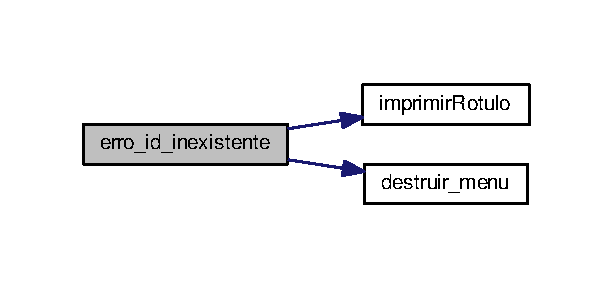
\includegraphics[width=294pt]{main_8cc_a8e3083a90f6cf70bdfd6abd70494c74e_cgraph}
\end{center}
\end{figure}




Este é o diagrama das funções que utilizam esta função\-:\nopagebreak
\begin{figure}[H]
\begin{center}
\leavevmode
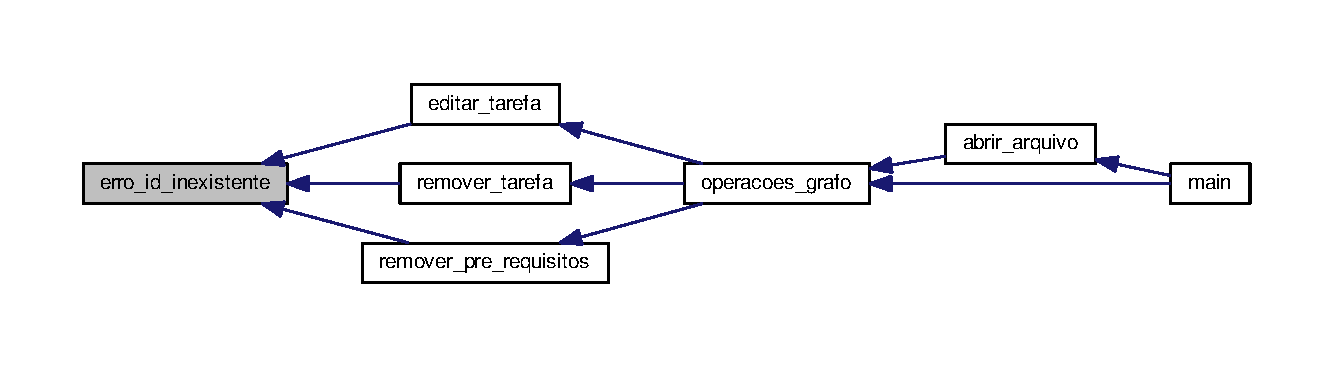
\includegraphics[width=350pt]{main_8cc_a8e3083a90f6cf70bdfd6abd70494c74e_icgraph}
\end{center}
\end{figure}


\hypertarget{main_8cc_acf899fb4107a26f962c26ec5292148cd}{\index{main.\-cc@{main.\-cc}!erro\-\_\-id\-\_\-invalido@{erro\-\_\-id\-\_\-invalido}}
\index{erro\-\_\-id\-\_\-invalido@{erro\-\_\-id\-\_\-invalido}!main.cc@{main.\-cc}}
\subsubsection[{erro\-\_\-id\-\_\-invalido}]{\setlength{\rightskip}{0pt plus 5cm}void erro\-\_\-id\-\_\-invalido (
\begin{DoxyParamCaption}
{}
\end{DoxyParamCaption}
)}}\label{main_8cc_acf899fb4107a26f962c26ec5292148cd}


Grafo de chamadas desta função\-:\nopagebreak
\begin{figure}[H]
\begin{center}
\leavevmode
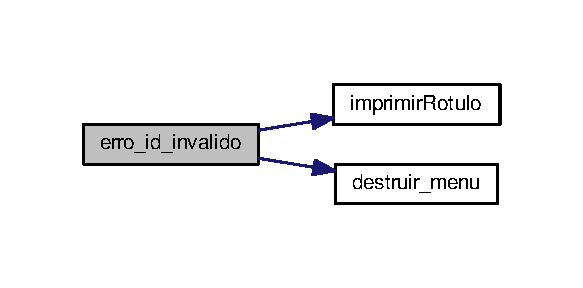
\includegraphics[width=280pt]{main_8cc_acf899fb4107a26f962c26ec5292148cd_cgraph}
\end{center}
\end{figure}




Este é o diagrama das funções que utilizam esta função\-:\nopagebreak
\begin{figure}[H]
\begin{center}
\leavevmode
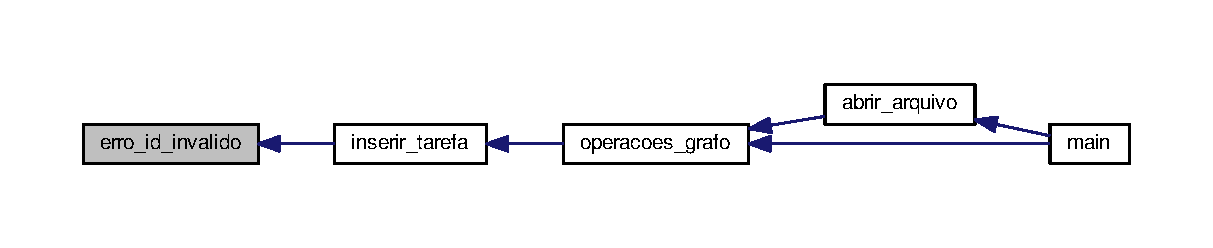
\includegraphics[width=350pt]{main_8cc_acf899fb4107a26f962c26ec5292148cd_icgraph}
\end{center}
\end{figure}


\hypertarget{main_8cc_aef0e5ebaf10f94ec3baf710468b2bca8}{\index{main.\-cc@{main.\-cc}!erro\-\_\-insere\-\_\-pre\-\_\-requisito@{erro\-\_\-insere\-\_\-pre\-\_\-requisito}}
\index{erro\-\_\-insere\-\_\-pre\-\_\-requisito@{erro\-\_\-insere\-\_\-pre\-\_\-requisito}!main.cc@{main.\-cc}}
\subsubsection[{erro\-\_\-insere\-\_\-pre\-\_\-requisito}]{\setlength{\rightskip}{0pt plus 5cm}void erro\-\_\-insere\-\_\-pre\-\_\-requisito (
\begin{DoxyParamCaption}
{}
\end{DoxyParamCaption}
)}}\label{main_8cc_aef0e5ebaf10f94ec3baf710468b2bca8}


Grafo de chamadas desta função\-:\nopagebreak
\begin{figure}[H]
\begin{center}
\leavevmode
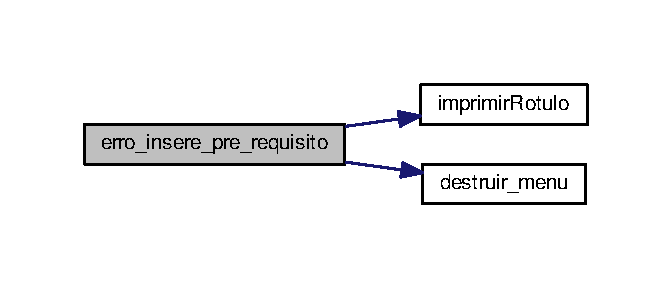
\includegraphics[width=322pt]{main_8cc_aef0e5ebaf10f94ec3baf710468b2bca8_cgraph}
\end{center}
\end{figure}




Este é o diagrama das funções que utilizam esta função\-:\nopagebreak
\begin{figure}[H]
\begin{center}
\leavevmode
\includegraphics[width=350pt]{main_8cc_aef0e5ebaf10f94ec3baf710468b2bca8_icgraph}
\end{center}
\end{figure}


\hypertarget{main_8cc_adcc550070c8292efdd63f7df8bbdd58a}{\index{main.\-cc@{main.\-cc}!filtrar\-\_\-tarefas\-\_\-completadas@{filtrar\-\_\-tarefas\-\_\-completadas}}
\index{filtrar\-\_\-tarefas\-\_\-completadas@{filtrar\-\_\-tarefas\-\_\-completadas}!main.cc@{main.\-cc}}
\subsubsection[{filtrar\-\_\-tarefas\-\_\-completadas}]{\setlength{\rightskip}{0pt plus 5cm}void filtrar\-\_\-tarefas\-\_\-completadas (
\begin{DoxyParamCaption}
\item[{{\bf grafo} $\ast$}]{G}
\end{DoxyParamCaption}
)}}\label{main_8cc_adcc550070c8292efdd63f7df8bbdd58a}


Grafo de chamadas desta função\-:\nopagebreak
\begin{figure}[H]
\begin{center}
\leavevmode
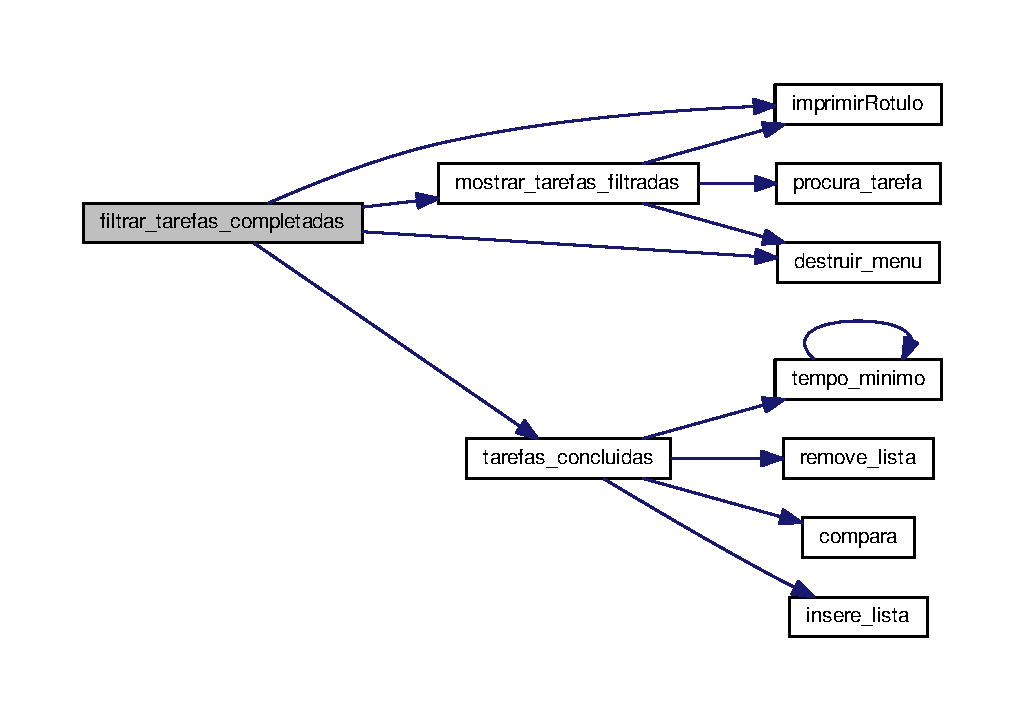
\includegraphics[width=350pt]{main_8cc_adcc550070c8292efdd63f7df8bbdd58a_cgraph}
\end{center}
\end{figure}




Este é o diagrama das funções que utilizam esta função\-:\nopagebreak
\begin{figure}[H]
\begin{center}
\leavevmode
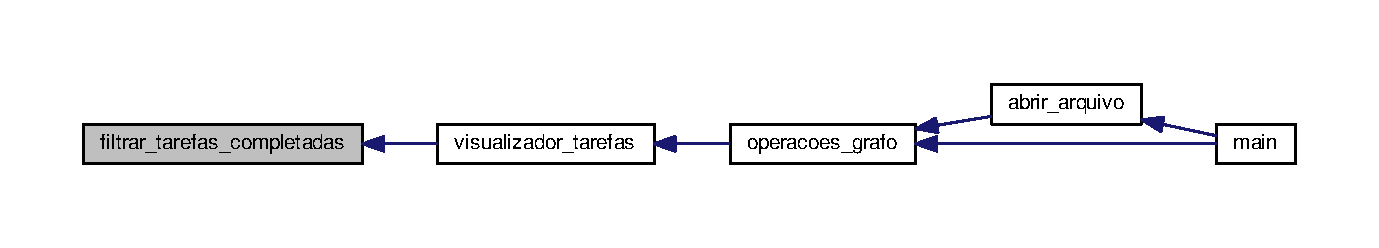
\includegraphics[width=350pt]{main_8cc_adcc550070c8292efdd63f7df8bbdd58a_icgraph}
\end{center}
\end{figure}


\hypertarget{main_8cc_af680447ac3023912e86df70f144373d8}{\index{main.\-cc@{main.\-cc}!importar\-\_\-de\-\_\-arquivo@{importar\-\_\-de\-\_\-arquivo}}
\index{importar\-\_\-de\-\_\-arquivo@{importar\-\_\-de\-\_\-arquivo}!main.cc@{main.\-cc}}
\subsubsection[{importar\-\_\-de\-\_\-arquivo}]{\setlength{\rightskip}{0pt plus 5cm}char$\ast$ importar\-\_\-de\-\_\-arquivo (
\begin{DoxyParamCaption}
\item[{char $\ast$}]{nome\-Arquivo}
\end{DoxyParamCaption}
)}}\label{main_8cc_af680447ac3023912e86df70f144373d8}


Grafo de chamadas desta função\-:\nopagebreak
\begin{figure}[H]
\begin{center}
\leavevmode
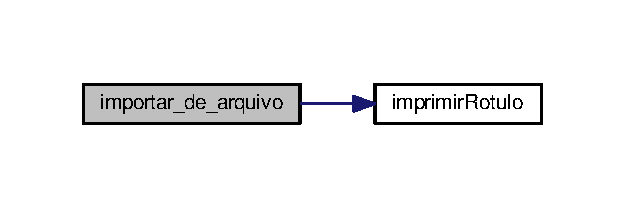
\includegraphics[width=300pt]{main_8cc_af680447ac3023912e86df70f144373d8_cgraph}
\end{center}
\end{figure}




Este é o diagrama das funções que utilizam esta função\-:\nopagebreak
\begin{figure}[H]
\begin{center}
\leavevmode
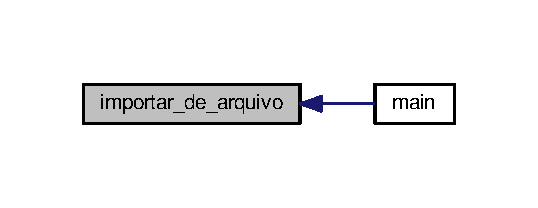
\includegraphics[width=258pt]{main_8cc_af680447ac3023912e86df70f144373d8_icgraph}
\end{center}
\end{figure}


\hypertarget{main_8cc_abc30d77428eefe83c569f49b7e48a7f8}{\index{main.\-cc@{main.\-cc}!imprimir\-\_\-em\-\_\-arquivo@{imprimir\-\_\-em\-\_\-arquivo}}
\index{imprimir\-\_\-em\-\_\-arquivo@{imprimir\-\_\-em\-\_\-arquivo}!main.cc@{main.\-cc}}
\subsubsection[{imprimir\-\_\-em\-\_\-arquivo}]{\setlength{\rightskip}{0pt plus 5cm}void imprimir\-\_\-em\-\_\-arquivo (
\begin{DoxyParamCaption}
\item[{{\bf grafo} $\ast$}]{G}
\end{DoxyParamCaption}
)}}\label{main_8cc_abc30d77428eefe83c569f49b7e48a7f8}


Grafo de chamadas desta função\-:\nopagebreak
\begin{figure}[H]
\begin{center}
\leavevmode
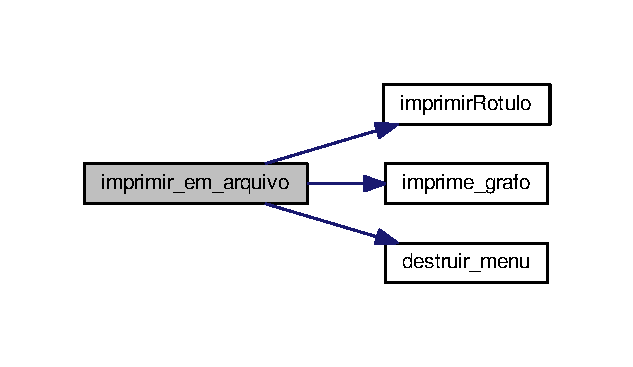
\includegraphics[width=304pt]{main_8cc_abc30d77428eefe83c569f49b7e48a7f8_cgraph}
\end{center}
\end{figure}




Este é o diagrama das funções que utilizam esta função\-:\nopagebreak
\begin{figure}[H]
\begin{center}
\leavevmode
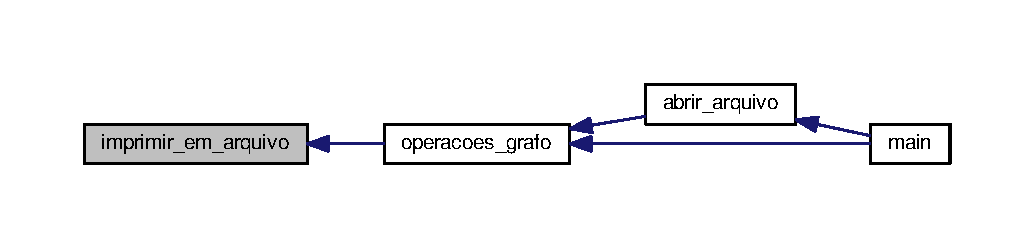
\includegraphics[width=350pt]{main_8cc_abc30d77428eefe83c569f49b7e48a7f8_icgraph}
\end{center}
\end{figure}


\hypertarget{main_8cc_ad2a06ffdf1033b3b1c11f337fa12553b}{\index{main.\-cc@{main.\-cc}!imprimir\-Rotulo@{imprimir\-Rotulo}}
\index{imprimir\-Rotulo@{imprimir\-Rotulo}!main.cc@{main.\-cc}}
\subsubsection[{imprimir\-Rotulo}]{\setlength{\rightskip}{0pt plus 5cm}void imprimir\-Rotulo (
\begin{DoxyParamCaption}
\item[{W\-I\-N\-D\-O\-W $\ast$}]{tmp\-Janela, }
\item[{int}]{y, }
\item[{int}]{x, }
\item[{char $\ast$}]{s\-Rotulo}
\end{DoxyParamCaption}
)}}\label{main_8cc_ad2a06ffdf1033b3b1c11f337fa12553b}


Este é o diagrama das funções que utilizam esta função\-:\nopagebreak
\begin{figure}[H]
\begin{center}
\leavevmode
\includegraphics[width=350pt]{main_8cc_ad2a06ffdf1033b3b1c11f337fa12553b_icgraph}
\end{center}
\end{figure}


\hypertarget{main_8cc_a16c89e840263b1af21caf3211b6640b2}{\index{main.\-cc@{main.\-cc}!inserir\-\_\-novo\-\_\-pre\-\_\-requisito@{inserir\-\_\-novo\-\_\-pre\-\_\-requisito}}
\index{inserir\-\_\-novo\-\_\-pre\-\_\-requisito@{inserir\-\_\-novo\-\_\-pre\-\_\-requisito}!main.cc@{main.\-cc}}
\subsubsection[{inserir\-\_\-novo\-\_\-pre\-\_\-requisito}]{\setlength{\rightskip}{0pt plus 5cm}{\bf grafo}$\ast$ inserir\-\_\-novo\-\_\-pre\-\_\-requisito (
\begin{DoxyParamCaption}
\item[{{\bf grafo} $\ast$}]{G}
\end{DoxyParamCaption}
)}}\label{main_8cc_a16c89e840263b1af21caf3211b6640b2}


Grafo de chamadas desta função\-:\nopagebreak
\begin{figure}[H]
\begin{center}
\leavevmode
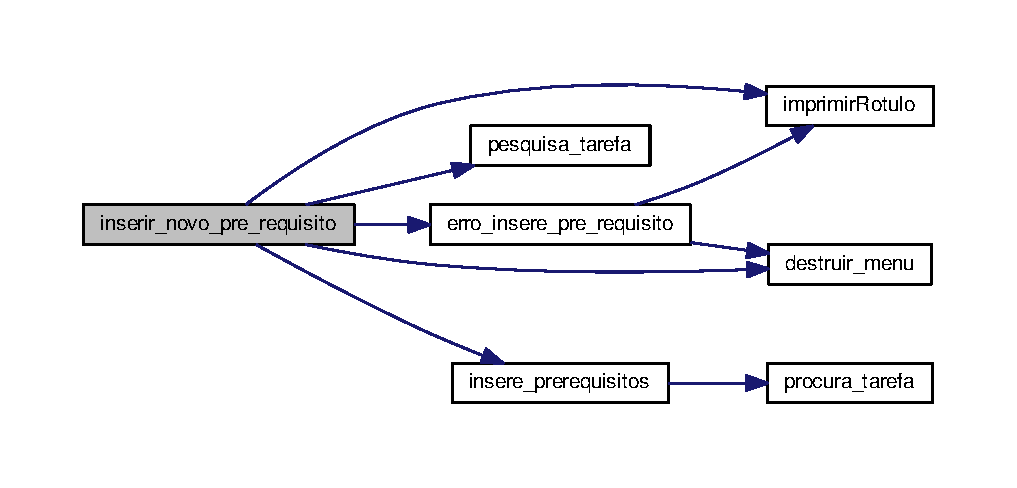
\includegraphics[width=350pt]{main_8cc_a16c89e840263b1af21caf3211b6640b2_cgraph}
\end{center}
\end{figure}




Este é o diagrama das funções que utilizam esta função\-:\nopagebreak
\begin{figure}[H]
\begin{center}
\leavevmode
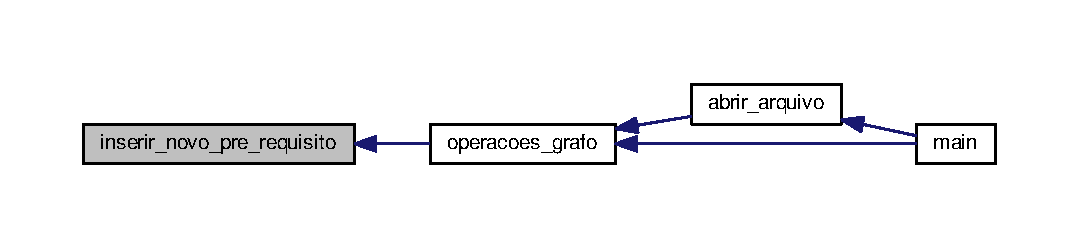
\includegraphics[width=350pt]{main_8cc_a16c89e840263b1af21caf3211b6640b2_icgraph}
\end{center}
\end{figure}


\hypertarget{main_8cc_adb3b0c3b009c68f86673eb7bdeef601c}{\index{main.\-cc@{main.\-cc}!inserir\-\_\-tarefa@{inserir\-\_\-tarefa}}
\index{inserir\-\_\-tarefa@{inserir\-\_\-tarefa}!main.cc@{main.\-cc}}
\subsubsection[{inserir\-\_\-tarefa}]{\setlength{\rightskip}{0pt plus 5cm}{\bf grafo}$\ast$ inserir\-\_\-tarefa (
\begin{DoxyParamCaption}
\item[{{\bf grafo} $\ast$}]{G}
\end{DoxyParamCaption}
)}}\label{main_8cc_adb3b0c3b009c68f86673eb7bdeef601c}


Grafo de chamadas desta função\-:\nopagebreak
\begin{figure}[H]
\begin{center}
\leavevmode
\includegraphics[width=350pt]{main_8cc_adb3b0c3b009c68f86673eb7bdeef601c_cgraph}
\end{center}
\end{figure}




Este é o diagrama das funções que utilizam esta função\-:\nopagebreak
\begin{figure}[H]
\begin{center}
\leavevmode
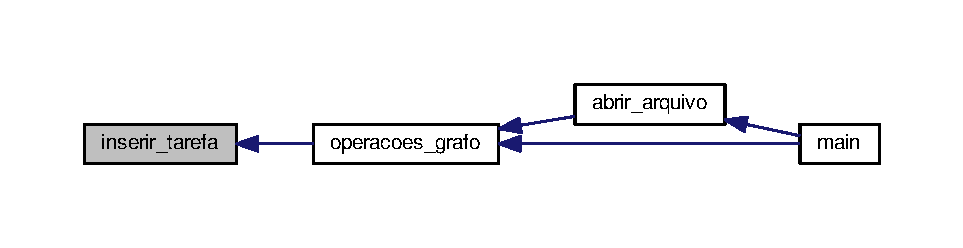
\includegraphics[width=350pt]{main_8cc_adb3b0c3b009c68f86673eb7bdeef601c_icgraph}
\end{center}
\end{figure}


\hypertarget{main_8cc_ae66f6b31b5ad750f1fe042a706a4e3d4}{\index{main.\-cc@{main.\-cc}!main@{main}}
\index{main@{main}!main.cc@{main.\-cc}}
\subsubsection[{main}]{\setlength{\rightskip}{0pt plus 5cm}int main (
\begin{DoxyParamCaption}
{}
\end{DoxyParamCaption}
)}}\label{main_8cc_ae66f6b31b5ad750f1fe042a706a4e3d4}


Grafo de chamadas desta função\-:\nopagebreak
\begin{figure}[H]
\begin{center}
\leavevmode
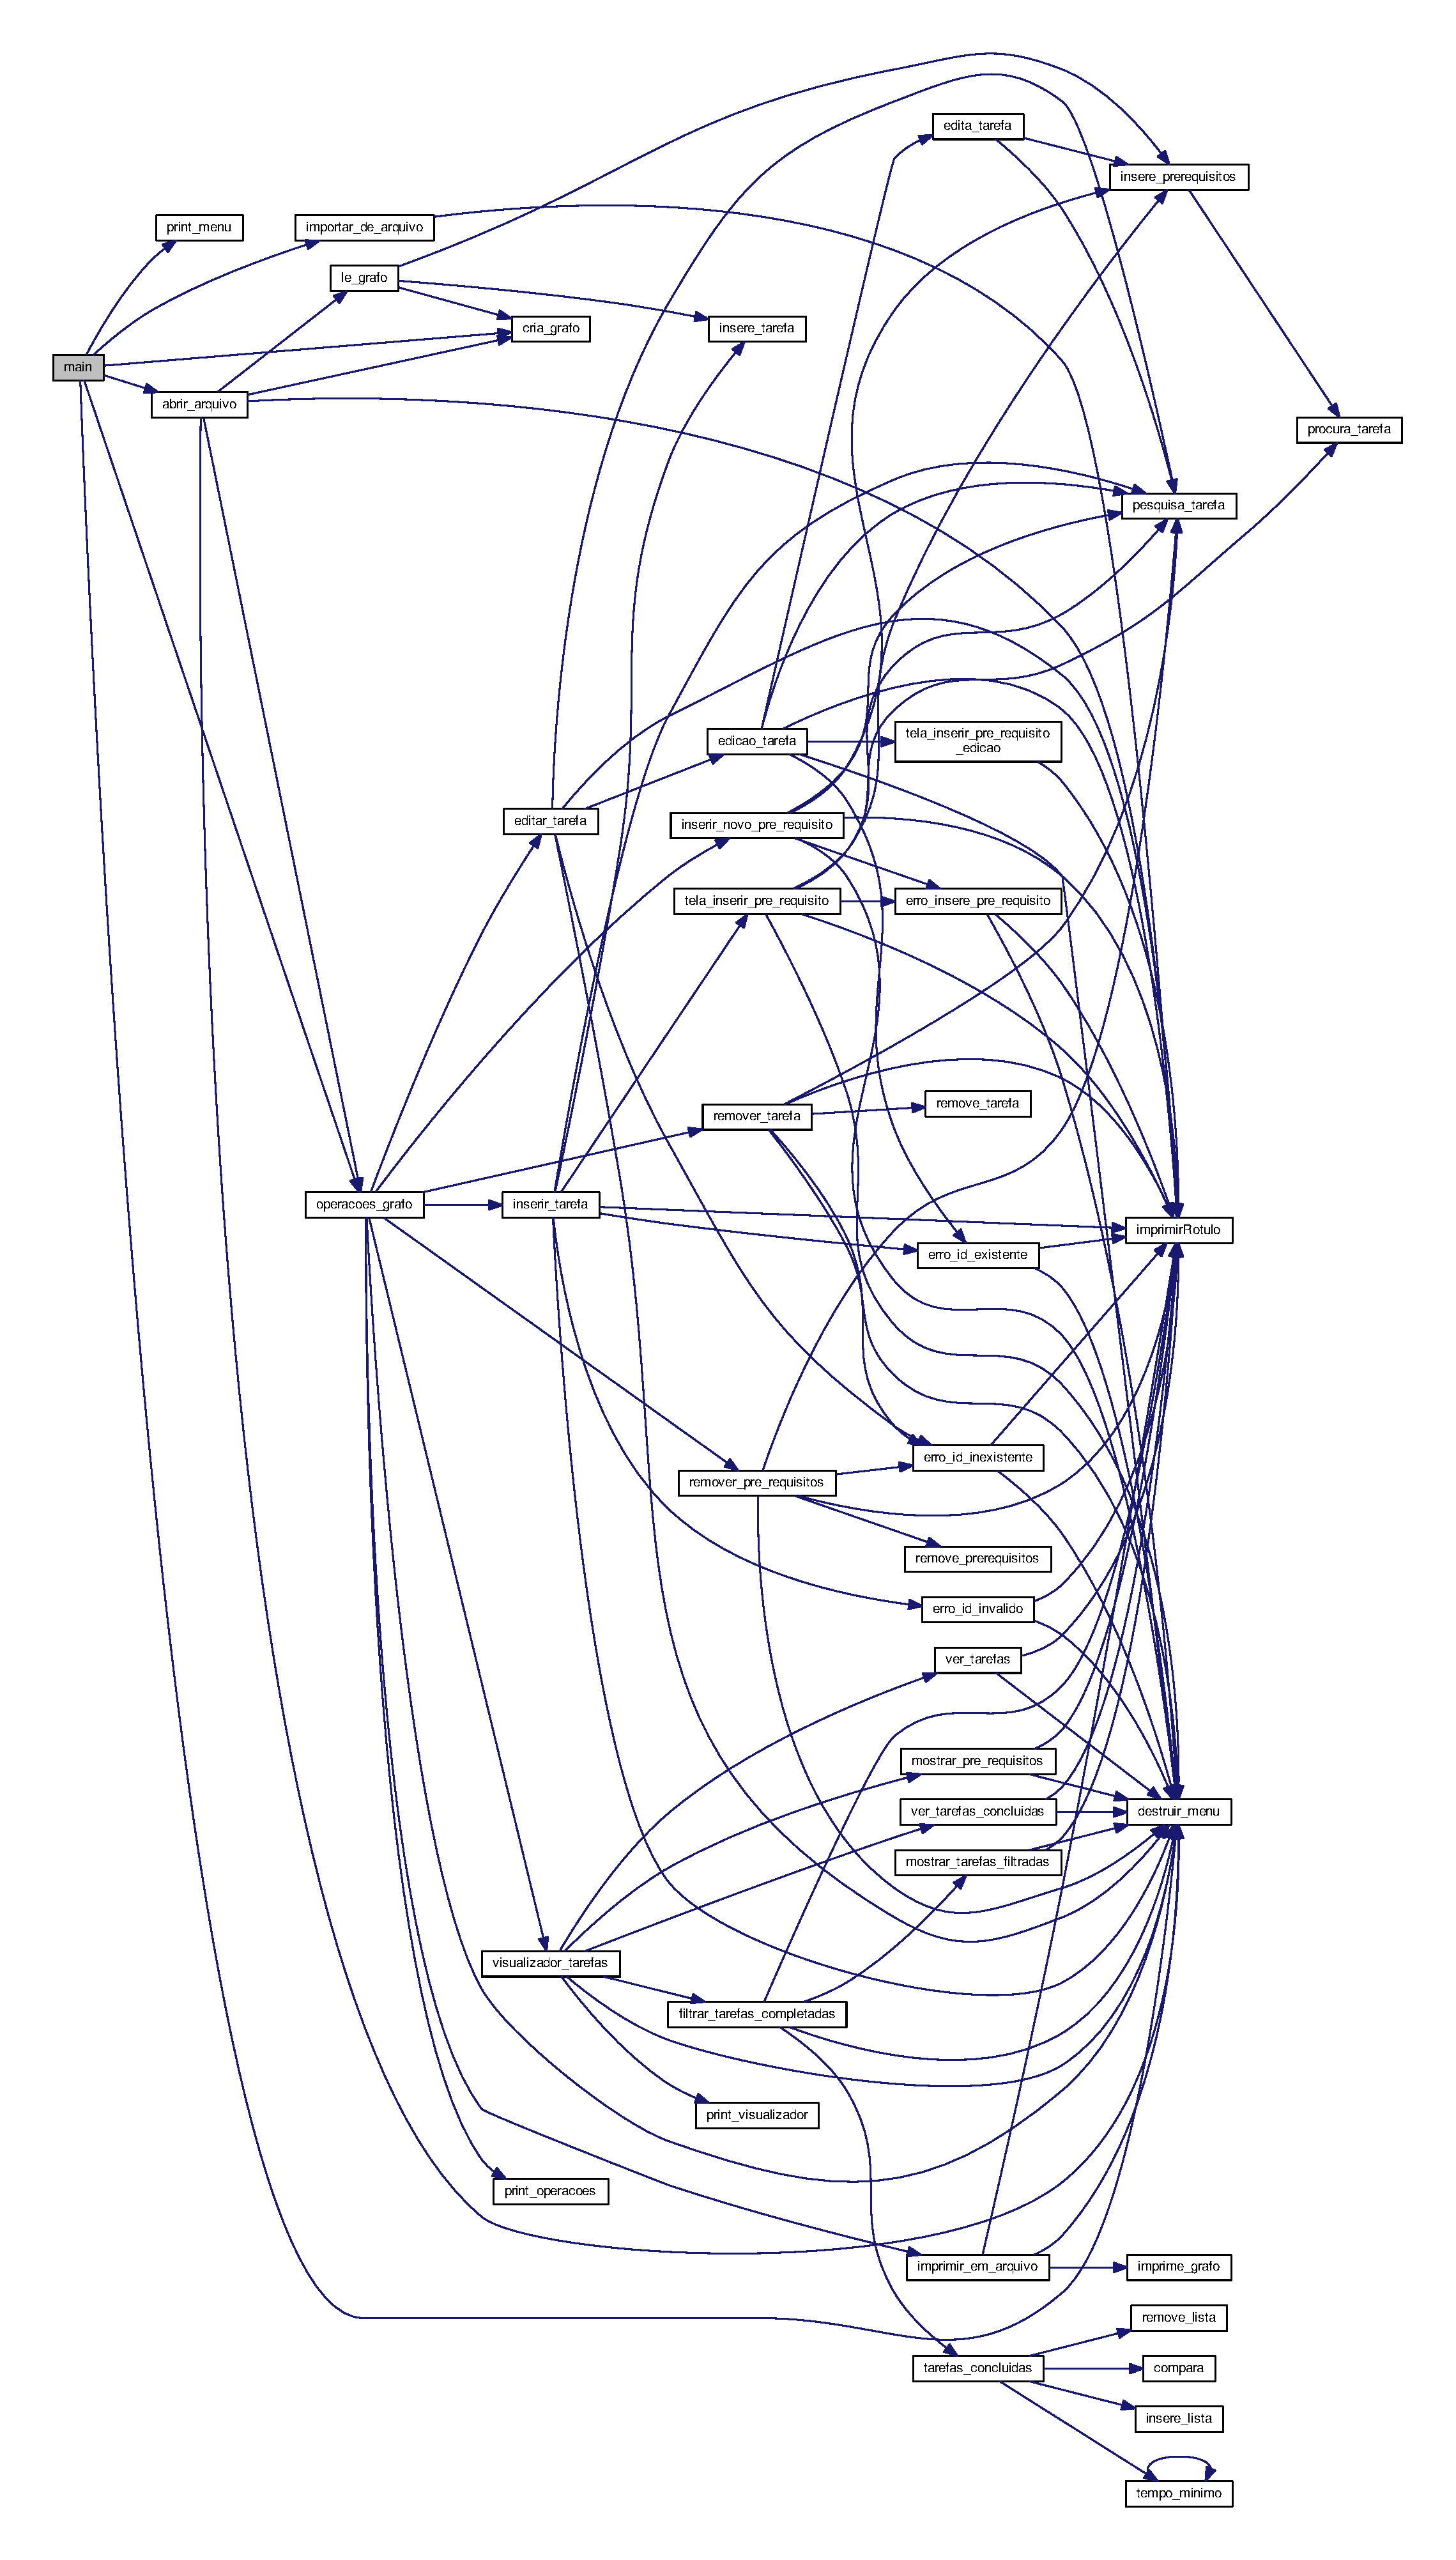
\includegraphics[height=550pt]{main_8cc_ae66f6b31b5ad750f1fe042a706a4e3d4_cgraph}
\end{center}
\end{figure}


\hypertarget{main_8cc_a4f8f29b1eba21e0b51992f8de173a582}{\index{main.\-cc@{main.\-cc}!mostrar\-\_\-pre\-\_\-requisitos@{mostrar\-\_\-pre\-\_\-requisitos}}
\index{mostrar\-\_\-pre\-\_\-requisitos@{mostrar\-\_\-pre\-\_\-requisitos}!main.cc@{main.\-cc}}
\subsubsection[{mostrar\-\_\-pre\-\_\-requisitos}]{\setlength{\rightskip}{0pt plus 5cm}void mostrar\-\_\-pre\-\_\-requisitos (
\begin{DoxyParamCaption}
\item[{{\bf grafo} $\ast$}]{G}
\end{DoxyParamCaption}
)}}\label{main_8cc_a4f8f29b1eba21e0b51992f8de173a582}


Grafo de chamadas desta função\-:\nopagebreak
\begin{figure}[H]
\begin{center}
\leavevmode
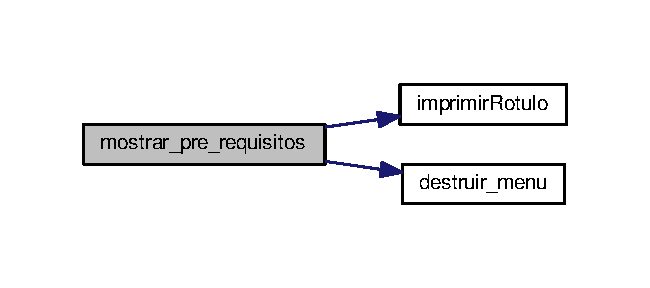
\includegraphics[width=312pt]{main_8cc_a4f8f29b1eba21e0b51992f8de173a582_cgraph}
\end{center}
\end{figure}




Este é o diagrama das funções que utilizam esta função\-:\nopagebreak
\begin{figure}[H]
\begin{center}
\leavevmode
\includegraphics[width=350pt]{main_8cc_a4f8f29b1eba21e0b51992f8de173a582_icgraph}
\end{center}
\end{figure}


\hypertarget{main_8cc_aaaa25a5b0eda0fab944a03026249b324}{\index{main.\-cc@{main.\-cc}!mostrar\-\_\-tarefas\-\_\-filtradas@{mostrar\-\_\-tarefas\-\_\-filtradas}}
\index{mostrar\-\_\-tarefas\-\_\-filtradas@{mostrar\-\_\-tarefas\-\_\-filtradas}!main.cc@{main.\-cc}}
\subsubsection[{mostrar\-\_\-tarefas\-\_\-filtradas}]{\setlength{\rightskip}{0pt plus 5cm}void mostrar\-\_\-tarefas\-\_\-filtradas (
\begin{DoxyParamCaption}
\item[{{\bf grafo} $\ast$}]{G, }
\item[{int $\ast$}]{tarefas}
\end{DoxyParamCaption}
)}}\label{main_8cc_aaaa25a5b0eda0fab944a03026249b324}


Grafo de chamadas desta função\-:\nopagebreak
\begin{figure}[H]
\begin{center}
\leavevmode
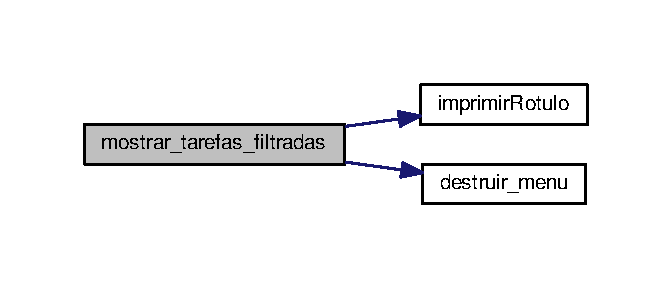
\includegraphics[width=322pt]{main_8cc_aaaa25a5b0eda0fab944a03026249b324_cgraph}
\end{center}
\end{figure}




Este é o diagrama das funções que utilizam esta função\-:\nopagebreak
\begin{figure}[H]
\begin{center}
\leavevmode
\includegraphics[width=350pt]{main_8cc_aaaa25a5b0eda0fab944a03026249b324_icgraph}
\end{center}
\end{figure}


\hypertarget{main_8cc_af852bc15cf3d5217386a9bb0bf3b9abd}{\index{main.\-cc@{main.\-cc}!operacoes\-\_\-grafo@{operacoes\-\_\-grafo}}
\index{operacoes\-\_\-grafo@{operacoes\-\_\-grafo}!main.cc@{main.\-cc}}
\subsubsection[{operacoes\-\_\-grafo}]{\setlength{\rightskip}{0pt plus 5cm}{\bf grafo}$\ast$ operacoes\-\_\-grafo (
\begin{DoxyParamCaption}
\item[{{\bf grafo} $\ast$}]{G}
\end{DoxyParamCaption}
)}}\label{main_8cc_af852bc15cf3d5217386a9bb0bf3b9abd}


Grafo de chamadas desta função\-:\nopagebreak
\begin{figure}[H]
\begin{center}
\leavevmode
\includegraphics[height=550pt]{main_8cc_af852bc15cf3d5217386a9bb0bf3b9abd_cgraph}
\end{center}
\end{figure}




Este é o diagrama das funções que utilizam esta função\-:\nopagebreak
\begin{figure}[H]
\begin{center}
\leavevmode
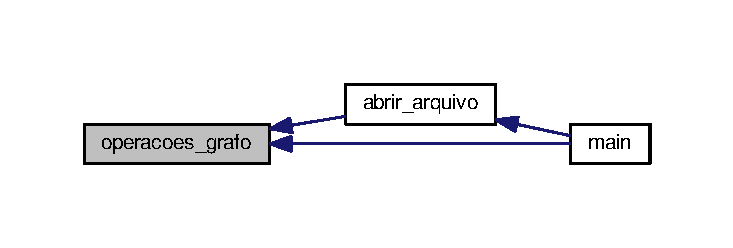
\includegraphics[width=350pt]{main_8cc_af852bc15cf3d5217386a9bb0bf3b9abd_icgraph}
\end{center}
\end{figure}


\hypertarget{main_8cc_a810164b29b6ded682dff19d56ec8e4b0}{\index{main.\-cc@{main.\-cc}!print\-\_\-menu@{print\-\_\-menu}}
\index{print\-\_\-menu@{print\-\_\-menu}!main.cc@{main.\-cc}}
\subsubsection[{print\-\_\-menu}]{\setlength{\rightskip}{0pt plus 5cm}void print\-\_\-menu (
\begin{DoxyParamCaption}
\item[{W\-I\-N\-D\-O\-W $\ast$}]{menu\-\_\-win, }
\item[{int}]{highlight}
\end{DoxyParamCaption}
)}}\label{main_8cc_a810164b29b6ded682dff19d56ec8e4b0}


Este é o diagrama das funções que utilizam esta função\-:\nopagebreak
\begin{figure}[H]
\begin{center}
\leavevmode
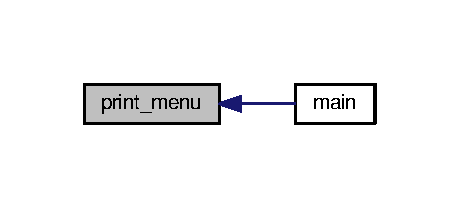
\includegraphics[width=220pt]{main_8cc_a810164b29b6ded682dff19d56ec8e4b0_icgraph}
\end{center}
\end{figure}


\hypertarget{main_8cc_a8b39b6c1f4d3623c384e80826e5b633e}{\index{main.\-cc@{main.\-cc}!print\-\_\-operacoes@{print\-\_\-operacoes}}
\index{print\-\_\-operacoes@{print\-\_\-operacoes}!main.cc@{main.\-cc}}
\subsubsection[{print\-\_\-operacoes}]{\setlength{\rightskip}{0pt plus 5cm}void print\-\_\-operacoes (
\begin{DoxyParamCaption}
\item[{W\-I\-N\-D\-O\-W $\ast$}]{menu\-\_\-win, }
\item[{int}]{highlight}
\end{DoxyParamCaption}
)}}\label{main_8cc_a8b39b6c1f4d3623c384e80826e5b633e}


Este é o diagrama das funções que utilizam esta função\-:\nopagebreak
\begin{figure}[H]
\begin{center}
\leavevmode
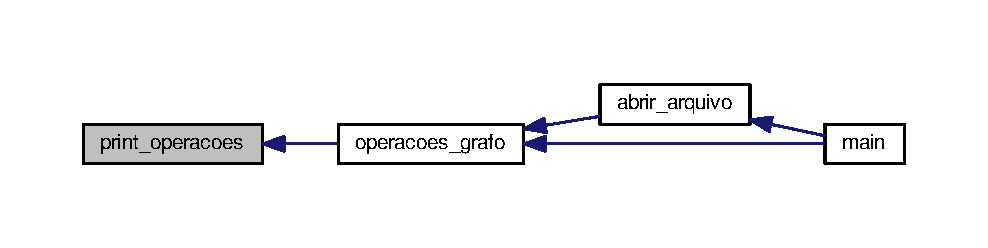
\includegraphics[width=350pt]{main_8cc_a8b39b6c1f4d3623c384e80826e5b633e_icgraph}
\end{center}
\end{figure}


\hypertarget{main_8cc_a4611d53166aabe6d0fb24bcfd407bd53}{\index{main.\-cc@{main.\-cc}!print\-\_\-visualizador@{print\-\_\-visualizador}}
\index{print\-\_\-visualizador@{print\-\_\-visualizador}!main.cc@{main.\-cc}}
\subsubsection[{print\-\_\-visualizador}]{\setlength{\rightskip}{0pt plus 5cm}void print\-\_\-visualizador (
\begin{DoxyParamCaption}
\item[{W\-I\-N\-D\-O\-W $\ast$}]{menu\-\_\-win, }
\item[{int}]{highlight}
\end{DoxyParamCaption}
)}}\label{main_8cc_a4611d53166aabe6d0fb24bcfd407bd53}


Este é o diagrama das funções que utilizam esta função\-:\nopagebreak
\begin{figure}[H]
\begin{center}
\leavevmode
\includegraphics[width=350pt]{main_8cc_a4611d53166aabe6d0fb24bcfd407bd53_icgraph}
\end{center}
\end{figure}


\hypertarget{main_8cc_ae96b9adf5e390d1a516e3fe5164714cc}{\index{main.\-cc@{main.\-cc}!remover\-\_\-pre\-\_\-requisitos@{remover\-\_\-pre\-\_\-requisitos}}
\index{remover\-\_\-pre\-\_\-requisitos@{remover\-\_\-pre\-\_\-requisitos}!main.cc@{main.\-cc}}
\subsubsection[{remover\-\_\-pre\-\_\-requisitos}]{\setlength{\rightskip}{0pt plus 5cm}{\bf grafo}$\ast$ remover\-\_\-pre\-\_\-requisitos (
\begin{DoxyParamCaption}
\item[{{\bf grafo} $\ast$}]{G}
\end{DoxyParamCaption}
)}}\label{main_8cc_ae96b9adf5e390d1a516e3fe5164714cc}


Grafo de chamadas desta função\-:\nopagebreak
\begin{figure}[H]
\begin{center}
\leavevmode
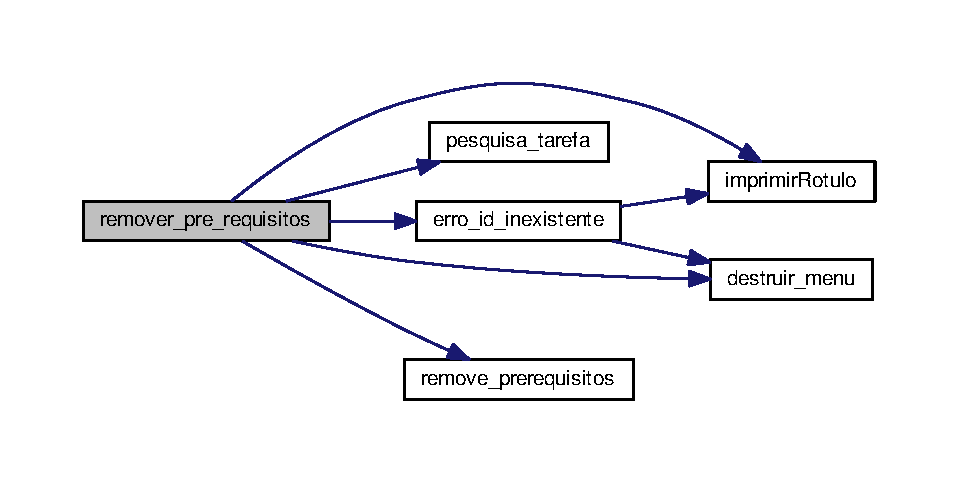
\includegraphics[width=350pt]{main_8cc_ae96b9adf5e390d1a516e3fe5164714cc_cgraph}
\end{center}
\end{figure}




Este é o diagrama das funções que utilizam esta função\-:\nopagebreak
\begin{figure}[H]
\begin{center}
\leavevmode
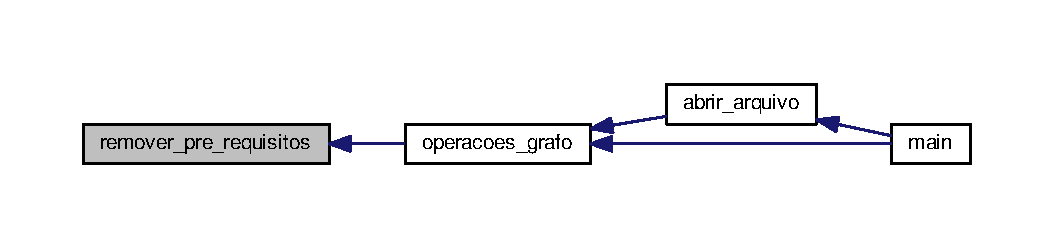
\includegraphics[width=350pt]{main_8cc_ae96b9adf5e390d1a516e3fe5164714cc_icgraph}
\end{center}
\end{figure}


\hypertarget{main_8cc_ab5f698491708904442d9d4f8583cd809}{\index{main.\-cc@{main.\-cc}!remover\-\_\-tarefa@{remover\-\_\-tarefa}}
\index{remover\-\_\-tarefa@{remover\-\_\-tarefa}!main.cc@{main.\-cc}}
\subsubsection[{remover\-\_\-tarefa}]{\setlength{\rightskip}{0pt plus 5cm}{\bf grafo}$\ast$ remover\-\_\-tarefa (
\begin{DoxyParamCaption}
\item[{{\bf grafo} $\ast$}]{G}
\end{DoxyParamCaption}
)}}\label{main_8cc_ab5f698491708904442d9d4f8583cd809}


Grafo de chamadas desta função\-:\nopagebreak
\begin{figure}[H]
\begin{center}
\leavevmode
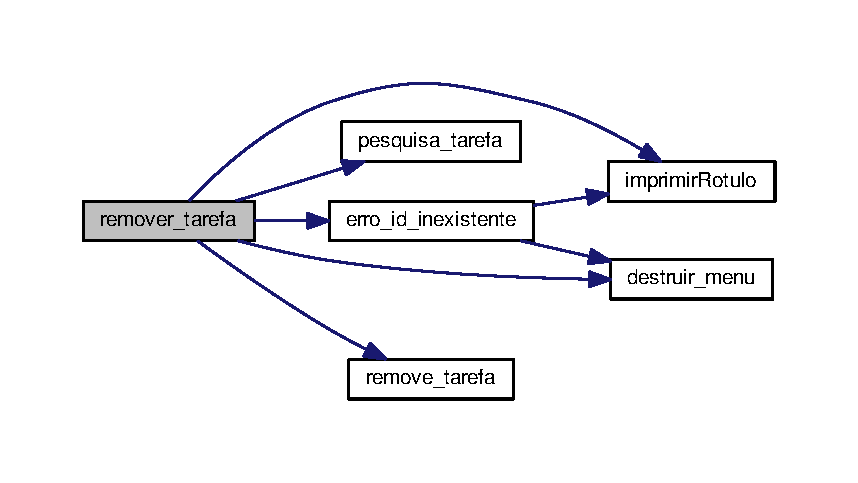
\includegraphics[width=350pt]{main_8cc_ab5f698491708904442d9d4f8583cd809_cgraph}
\end{center}
\end{figure}




Este é o diagrama das funções que utilizam esta função\-:\nopagebreak
\begin{figure}[H]
\begin{center}
\leavevmode
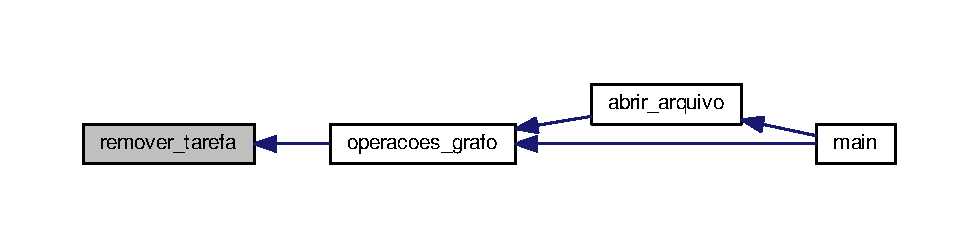
\includegraphics[width=350pt]{main_8cc_ab5f698491708904442d9d4f8583cd809_icgraph}
\end{center}
\end{figure}


\hypertarget{main_8cc_a5c0ceb9634231b92e0dfc9db33b727fa}{\index{main.\-cc@{main.\-cc}!tela\-\_\-inserir\-\_\-pre\-\_\-requisito@{tela\-\_\-inserir\-\_\-pre\-\_\-requisito}}
\index{tela\-\_\-inserir\-\_\-pre\-\_\-requisito@{tela\-\_\-inserir\-\_\-pre\-\_\-requisito}!main.cc@{main.\-cc}}
\subsubsection[{tela\-\_\-inserir\-\_\-pre\-\_\-requisito}]{\setlength{\rightskip}{0pt plus 5cm}{\bf grafo}$\ast$ tela\-\_\-inserir\-\_\-pre\-\_\-requisito (
\begin{DoxyParamCaption}
\item[{{\bf grafo} $\ast$}]{G, }
\item[{int}]{n\-\_\-prerequisitos, }
\item[{int}]{id\-\_\-tarefa}
\end{DoxyParamCaption}
)}}\label{main_8cc_a5c0ceb9634231b92e0dfc9db33b727fa}


Grafo de chamadas desta função\-:\nopagebreak
\begin{figure}[H]
\begin{center}
\leavevmode
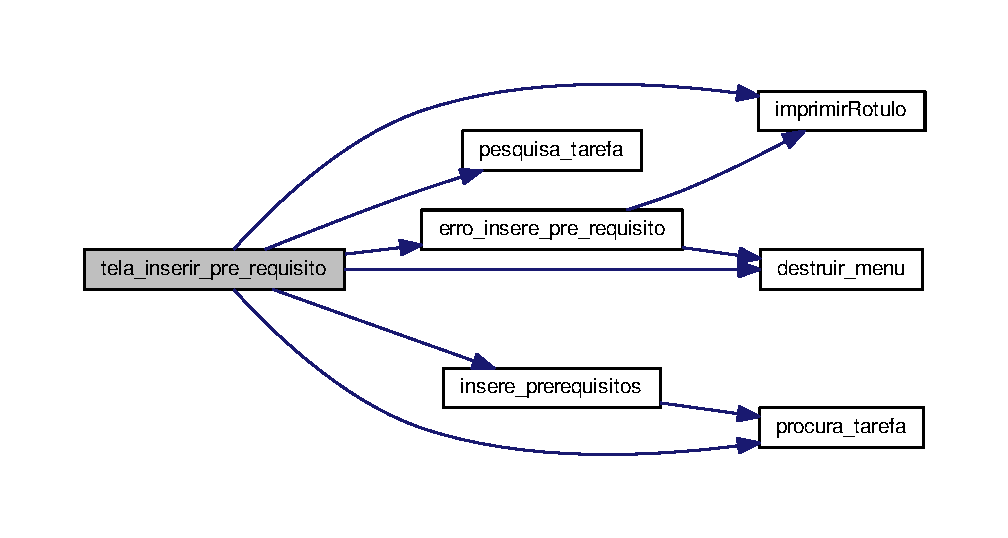
\includegraphics[width=350pt]{main_8cc_a5c0ceb9634231b92e0dfc9db33b727fa_cgraph}
\end{center}
\end{figure}




Este é o diagrama das funções que utilizam esta função\-:\nopagebreak
\begin{figure}[H]
\begin{center}
\leavevmode
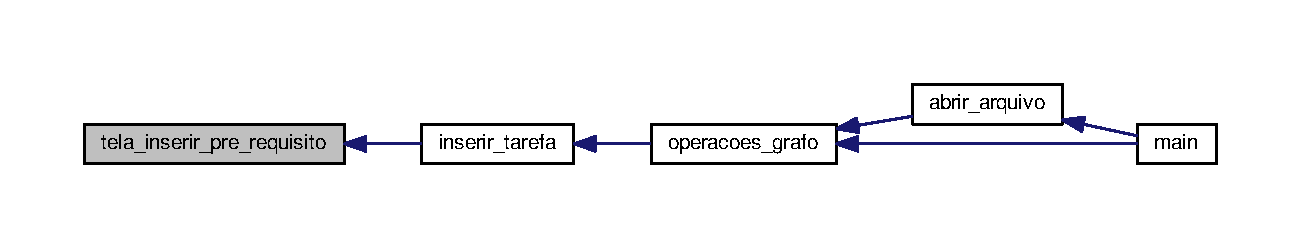
\includegraphics[width=350pt]{main_8cc_a5c0ceb9634231b92e0dfc9db33b727fa_icgraph}
\end{center}
\end{figure}


\hypertarget{main_8cc_a5f90fb7a7aa9c2393d70b4f95d675955}{\index{main.\-cc@{main.\-cc}!tela\-\_\-inserir\-\_\-pre\-\_\-requisito\-\_\-edicao@{tela\-\_\-inserir\-\_\-pre\-\_\-requisito\-\_\-edicao}}
\index{tela\-\_\-inserir\-\_\-pre\-\_\-requisito\-\_\-edicao@{tela\-\_\-inserir\-\_\-pre\-\_\-requisito\-\_\-edicao}!main.cc@{main.\-cc}}
\subsubsection[{tela\-\_\-inserir\-\_\-pre\-\_\-requisito\-\_\-edicao}]{\setlength{\rightskip}{0pt plus 5cm}int tela\-\_\-inserir\-\_\-pre\-\_\-requisito\-\_\-edicao (
\begin{DoxyParamCaption}
{}
\end{DoxyParamCaption}
)}}\label{main_8cc_a5f90fb7a7aa9c2393d70b4f95d675955}


Grafo de chamadas desta função\-:\nopagebreak
\begin{figure}[H]
\begin{center}
\leavevmode
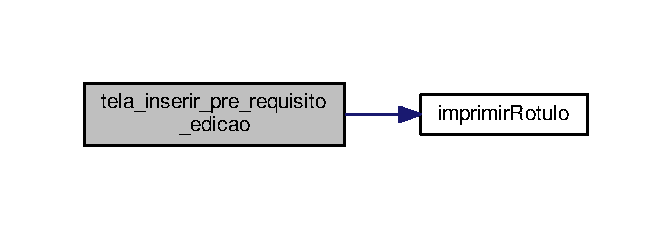
\includegraphics[width=322pt]{main_8cc_a5f90fb7a7aa9c2393d70b4f95d675955_cgraph}
\end{center}
\end{figure}




Este é o diagrama das funções que utilizam esta função\-:\nopagebreak
\begin{figure}[H]
\begin{center}
\leavevmode
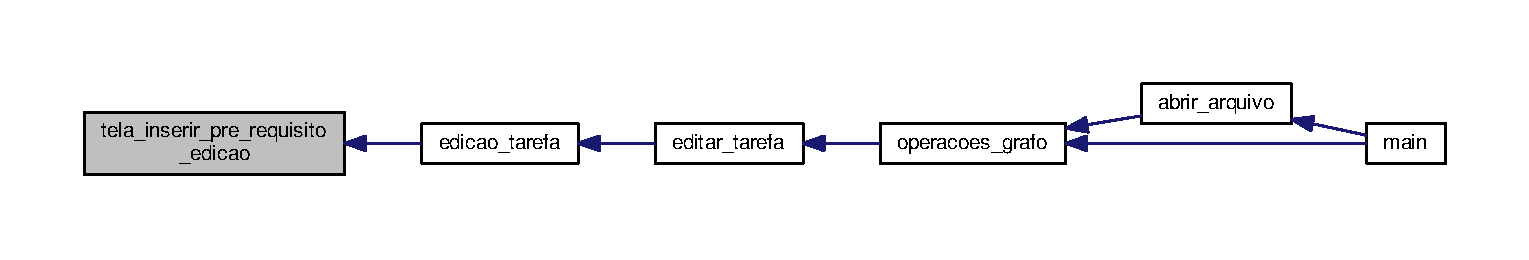
\includegraphics[width=350pt]{main_8cc_a5f90fb7a7aa9c2393d70b4f95d675955_icgraph}
\end{center}
\end{figure}


\hypertarget{main_8cc_aa0ac4a2d1125c89ec5acc37dfde748c6}{\index{main.\-cc@{main.\-cc}!ver\-\_\-tarefas@{ver\-\_\-tarefas}}
\index{ver\-\_\-tarefas@{ver\-\_\-tarefas}!main.cc@{main.\-cc}}
\subsubsection[{ver\-\_\-tarefas}]{\setlength{\rightskip}{0pt plus 5cm}void ver\-\_\-tarefas (
\begin{DoxyParamCaption}
\item[{{\bf grafo} $\ast$}]{G}
\end{DoxyParamCaption}
)}}\label{main_8cc_aa0ac4a2d1125c89ec5acc37dfde748c6}


Grafo de chamadas desta função\-:\nopagebreak
\begin{figure}[H]
\begin{center}
\leavevmode
\includegraphics[width=262pt]{main_8cc_aa0ac4a2d1125c89ec5acc37dfde748c6_cgraph}
\end{center}
\end{figure}




Este é o diagrama das funções que utilizam esta função\-:\nopagebreak
\begin{figure}[H]
\begin{center}
\leavevmode
\includegraphics[width=350pt]{main_8cc_aa0ac4a2d1125c89ec5acc37dfde748c6_icgraph}
\end{center}
\end{figure}


\hypertarget{main_8cc_ab05b93d97a47c67aab51426cdad29a86}{\index{main.\-cc@{main.\-cc}!ver\-\_\-tarefas\-\_\-concluidas@{ver\-\_\-tarefas\-\_\-concluidas}}
\index{ver\-\_\-tarefas\-\_\-concluidas@{ver\-\_\-tarefas\-\_\-concluidas}!main.cc@{main.\-cc}}
\subsubsection[{ver\-\_\-tarefas\-\_\-concluidas}]{\setlength{\rightskip}{0pt plus 5cm}void ver\-\_\-tarefas\-\_\-concluidas (
\begin{DoxyParamCaption}
\item[{{\bf grafo} $\ast$}]{G}
\end{DoxyParamCaption}
)}}\label{main_8cc_ab05b93d97a47c67aab51426cdad29a86}


Grafo de chamadas desta função\-:\nopagebreak
\begin{figure}[H]
\begin{center}
\leavevmode
\includegraphics[width=314pt]{main_8cc_ab05b93d97a47c67aab51426cdad29a86_cgraph}
\end{center}
\end{figure}




Este é o diagrama das funções que utilizam esta função\-:\nopagebreak
\begin{figure}[H]
\begin{center}
\leavevmode
\includegraphics[width=350pt]{main_8cc_ab05b93d97a47c67aab51426cdad29a86_icgraph}
\end{center}
\end{figure}


\hypertarget{main_8cc_a5d247f6e8ee275a8cd007f922ae2acb3}{\index{main.\-cc@{main.\-cc}!visualizador\-\_\-tarefas@{visualizador\-\_\-tarefas}}
\index{visualizador\-\_\-tarefas@{visualizador\-\_\-tarefas}!main.cc@{main.\-cc}}
\subsubsection[{visualizador\-\_\-tarefas}]{\setlength{\rightskip}{0pt plus 5cm}void visualizador\-\_\-tarefas (
\begin{DoxyParamCaption}
\item[{{\bf grafo} $\ast$}]{G}
\end{DoxyParamCaption}
)}}\label{main_8cc_a5d247f6e8ee275a8cd007f922ae2acb3}


Grafo de chamadas desta função\-:\nopagebreak
\begin{figure}[H]
\begin{center}
\leavevmode
\includegraphics[width=350pt]{main_8cc_a5d247f6e8ee275a8cd007f922ae2acb3_cgraph}
\end{center}
\end{figure}




Este é o diagrama das funções que utilizam esta função\-:\nopagebreak
\begin{figure}[H]
\begin{center}
\leavevmode
\includegraphics[width=350pt]{main_8cc_a5d247f6e8ee275a8cd007f922ae2acb3_icgraph}
\end{center}
\end{figure}




\subsection{Documentação das variáveis}
\hypertarget{main_8cc_a24167c503992e21d9d3b767742346d4b}{\index{main.\-cc@{main.\-cc}!n\-\_\-opcoes@{n\-\_\-opcoes}}
\index{n\-\_\-opcoes@{n\-\_\-opcoes}!main.cc@{main.\-cc}}
\subsubsection[{n\-\_\-opcoes}]{\setlength{\rightskip}{0pt plus 5cm}int n\-\_\-opcoes = 3}}\label{main_8cc_a24167c503992e21d9d3b767742346d4b}
\hypertarget{main_8cc_a4e96567620b8107a3844f6a3b5860c74}{\index{main.\-cc@{main.\-cc}!n\-\_\-operacoes@{n\-\_\-operacoes}}
\index{n\-\_\-operacoes@{n\-\_\-operacoes}!main.cc@{main.\-cc}}
\subsubsection[{n\-\_\-operacoes}]{\setlength{\rightskip}{0pt plus 5cm}int n\-\_\-operacoes = 8}}\label{main_8cc_a4e96567620b8107a3844f6a3b5860c74}
\hypertarget{main_8cc_a44042648455eb7c48a35466047cd5911}{\index{main.\-cc@{main.\-cc}!n\-\_\-visualizador@{n\-\_\-visualizador}}
\index{n\-\_\-visualizador@{n\-\_\-visualizador}!main.cc@{main.\-cc}}
\subsubsection[{n\-\_\-visualizador}]{\setlength{\rightskip}{0pt plus 5cm}int n\-\_\-visualizador = 6}}\label{main_8cc_a44042648455eb7c48a35466047cd5911}
\hypertarget{main_8cc_a8f0744c55ee97ebf34757f8499a66139}{\index{main.\-cc@{main.\-cc}!startx@{startx}}
\index{startx@{startx}!main.cc@{main.\-cc}}
\subsubsection[{startx}]{\setlength{\rightskip}{0pt plus 5cm}int startx = 0}}\label{main_8cc_a8f0744c55ee97ebf34757f8499a66139}
\hypertarget{main_8cc_a19e264821cbd530471c1cf985d7cd239}{\index{main.\-cc@{main.\-cc}!starty@{starty}}
\index{starty@{starty}!main.cc@{main.\-cc}}
\subsubsection[{starty}]{\setlength{\rightskip}{0pt plus 5cm}int starty = 0}}\label{main_8cc_a19e264821cbd530471c1cf985d7cd239}
\hypertarget{main_8cc_a7e3eb983c89b73fc26206eb49d9e53f6}{\index{main.\-cc@{main.\-cc}!v\-Opcoes@{v\-Opcoes}}
\index{v\-Opcoes@{v\-Opcoes}!main.cc@{main.\-cc}}
\subsubsection[{v\-Opcoes}]{\setlength{\rightskip}{0pt plus 5cm}char v\-Opcoes\mbox{[}3\mbox{]}\mbox{[}70\mbox{]}}}\label{main_8cc_a7e3eb983c89b73fc26206eb49d9e53f6}
\hypertarget{main_8cc_a282382d81ff49bb355edf4b0e0c33ab5}{\index{main.\-cc@{main.\-cc}!v\-Operacoes@{v\-Operacoes}}
\index{v\-Operacoes@{v\-Operacoes}!main.cc@{main.\-cc}}
\subsubsection[{v\-Operacoes}]{\setlength{\rightskip}{0pt plus 5cm}char v\-Operacoes\mbox{[}8\mbox{]}\mbox{[}70\mbox{]}}}\label{main_8cc_a282382d81ff49bb355edf4b0e0c33ab5}
\hypertarget{main_8cc_ac830448011ecd7178e23030edbff0311}{\index{main.\-cc@{main.\-cc}!v\-Visualizador@{v\-Visualizador}}
\index{v\-Visualizador@{v\-Visualizador}!main.cc@{main.\-cc}}
\subsubsection[{v\-Visualizador}]{\setlength{\rightskip}{0pt plus 5cm}char v\-Visualizador\mbox{[}6\mbox{]}\mbox{[}70\mbox{]}}}\label{main_8cc_ac830448011ecd7178e23030edbff0311}

\hypertarget{grafo_8h}{\section{Referência ao ficheiro include/grafo.h}
\label{grafo_8h}\index{include/grafo.\-h@{include/grafo.\-h}}
}
Este grafo mostra quais são os ficheiros que incluem directamente ou indirectamente este ficheiro\-:
\nopagebreak
\begin{figure}[H]
\begin{center}
\leavevmode
\includegraphics[width=350pt]{grafo_8h__dep__incl}
\end{center}
\end{figure}
\subsection*{Componentes}
\begin{DoxyCompactItemize}
\item 
struct \hyperlink{structPreRequisitos}{Pre\-Requisitos}
\item 
struct \hyperlink{structTarefa}{Tarefa}
\item 
struct \hyperlink{structGrafo}{Grafo}
\end{DoxyCompactItemize}
\subsection*{Macros}
\begin{DoxyCompactItemize}
\item 
\#define \hyperlink{grafo_8h_a5d28dfdab86222715d699097e8cd092f}{T\-A\-M\-\_\-\-S\-T\-R\-I\-N\-G}~100
\item 
\#define \hyperlink{grafo_8h_ada9d403038db083d1a9ee9287ec41b2d}{F\-L\-G\-\_\-\-N\-O\-M\-E}~0x1
\item 
\#define \hyperlink{grafo_8h_a1b685616433755135786d05ac1281c8f}{F\-L\-G\-\_\-\-E\-X\-E\-C}~0x2
\item 
\#define \hyperlink{grafo_8h_a5b92a45371c0e3c1e1ebd008ec618cc2}{F\-L\-G\-\_\-\-D\-U\-R\-A}~0x4
\item 
\#define \hyperlink{grafo_8h_a0729dac97648478b3462870f82dc8777}{F\-L\-G\-\_\-\-I\-N\-I\-C}~0x8
\item 
\#define \hyperlink{grafo_8h_aeee53140ed342a607f5a1193706e6837}{F\-L\-G\-\_\-\-P\-R\-E\-R}~0x10
\item 
\#define \hyperlink{grafo_8h_a81ff8ddd98e8fe2be09bd9af6c727173}{F\-L\-G\-\_\-\-I\-D\-T\-R}~0x20
\item 
\#define \hyperlink{grafo_8h_a9ec306f36d50c7375e74f0d1c55a3a67}{I\-N\-T\-\_\-\-M\-A\-X}~2147483647
\end{DoxyCompactItemize}
\subsection*{Definições de tipos}
\begin{DoxyCompactItemize}
\item 
typedef struct \hyperlink{structPreRequisitos}{Pre\-Requisitos} \hyperlink{grafo_8h_a8d260ebf15bfe9b5f9366d2245289e15}{prerequisitos}
\item 
typedef struct \hyperlink{structTarefa}{Tarefa} \hyperlink{grafo_8h_ab156210f10bb550f6d61bea964f08c22}{tarefa}
\item 
typedef struct \hyperlink{structGrafo}{Grafo} \hyperlink{grafo_8h_abfb99265d91141543f92efaec783231d}{grafo}
\end{DoxyCompactItemize}
\subsection*{Funções}
\begin{DoxyCompactItemize}
\item 
\hyperlink{grafo_8h_abfb99265d91141543f92efaec783231d}{grafo} $\ast$ \hyperlink{grafo_8h_aa0ebaaf04a0e9c455c6571246b5c1e15}{cria\-\_\-grafo} ()
\item 
\hyperlink{grafo_8h_abfb99265d91141543f92efaec783231d}{grafo} $\ast$ \hyperlink{grafo_8h_a563a8912631e461ec1d9a2bff50426d9}{insere\-\_\-tarefa} (\hyperlink{grafo_8h_abfb99265d91141543f92efaec783231d}{grafo} $\ast$G, int id\-\_\-tarefa, char $\ast$nome\-\_\-tarefa, int tarefa\-\_\-executada, int duracao\-\_\-tarefa, int inicio\-\_\-min\-\_\-tarefa, int n\-\_\-prerequisitos)
\item 
\hyperlink{grafo_8h_abfb99265d91141543f92efaec783231d}{grafo} $\ast$ \hyperlink{grafo_8h_adaeb2e2aa0bf8a2fbb149376a33bd443}{edita\-\_\-tarefa} (\hyperlink{grafo_8h_abfb99265d91141543f92efaec783231d}{grafo} $\ast$G, int id\-\_\-tarefa, int novo\-\_\-id\-\_\-tarefa, char $\ast$nome\-\_\-tarefa, int tarefa\-\_\-executada, int duracao\-\_\-tarefa, int inicio\-\_\-min\-\_\-tarefa, int n\-\_\-prerequisitos, int $\ast$id\-\_\-prerequisitos, int flag)
\item 
\hyperlink{grafo_8h_abfb99265d91141543f92efaec783231d}{grafo} $\ast$ \hyperlink{grafo_8h_a3fe6389b74d0356a95800a3d29d7d664}{insere\-\_\-prerequisitos} (\hyperlink{grafo_8h_abfb99265d91141543f92efaec783231d}{grafo} $\ast$G, int id\-\_\-tarefa, int id\-\_\-prerequisito)
\item 
\hyperlink{grafo_8h_abfb99265d91141543f92efaec783231d}{grafo} $\ast$ \hyperlink{grafo_8h_abab0a8730861a86fe9a0713b3dcc018b}{remove\-\_\-tarefa} (\hyperlink{grafo_8h_abfb99265d91141543f92efaec783231d}{grafo} $\ast$G, int id\-\_\-tarefa)
\item 
\hyperlink{grafo_8h_abfb99265d91141543f92efaec783231d}{grafo} $\ast$ \hyperlink{grafo_8h_ad1f78512cd30c15264c68265f61296a6}{remove\-\_\-prerequisitos} (\hyperlink{grafo_8h_abfb99265d91141543f92efaec783231d}{grafo} $\ast$G, int id\-\_\-tarefa)
\item 
\hyperlink{grafo_8h_abfb99265d91141543f92efaec783231d}{grafo} $\ast$ \hyperlink{grafo_8h_a07e2bda52af22bd5988dfab266b696f3}{le\-\_\-grafo} (F\-I\-L\-E $\ast$fp)
\item 
void \hyperlink{grafo_8h_a64cc9fac8ef1d2aa018e1bad3e43d87e}{libera\-\_\-grafo} (\hyperlink{grafo_8h_abfb99265d91141543f92efaec783231d}{grafo} $\ast$G)
\item 
void \hyperlink{grafo_8h_ac7a63f8753e7dbbb4117e6d4ebaa5933}{imprime\-\_\-grafo} (\hyperlink{grafo_8h_abfb99265d91141543f92efaec783231d}{grafo} $\ast$G, char $\ast$nome\-\_\-arq)
\item 
int \hyperlink{grafo_8h_ad44b772951e7f095b7ad67dbddbc5404}{verifica\-\_\-consistencia} (\hyperlink{grafo_8h_abfb99265d91141543f92efaec783231d}{grafo} $\ast$G)
\item 
int \hyperlink{grafo_8h_a1e996ff4a17fa0e42fc8ff6bdc605dc1}{pesquisa\-\_\-tarefa} (\hyperlink{grafo_8h_abfb99265d91141543f92efaec783231d}{grafo} $\ast$G, int id\-\_\-tarefa)
\item 
int \hyperlink{grafo_8h_aacb0f98cd7a5b04836f1cffb745666f1}{pesquisa\-\_\-prerequisitos} (\hyperlink{grafo_8h_abfb99265d91141543f92efaec783231d}{grafo} $\ast$G, int id\-\_\-tarefa, int id\-\_\-prerequisito)
\item 
\hyperlink{grafo_8h_ab156210f10bb550f6d61bea964f08c22}{tarefa} $\ast$ \hyperlink{grafo_8h_a0e6585acadedc05719f93fa778cf1dcb}{procura\-\_\-tarefa} (\hyperlink{grafo_8h_abfb99265d91141543f92efaec783231d}{grafo} $\ast$G, int id\-\_\-tarefa)
\item 
int \hyperlink{grafo_8h_a6884bc1455bdfb3648b3e2514998e599}{tempo\-\_\-minimo} (\hyperlink{grafo_8h_abfb99265d91141543f92efaec783231d}{grafo} $\ast$G, int id\-\_\-tarefa)
\item 
int \hyperlink{grafo_8h_a57212202dfe77e7368840b67dd5fd46c}{tempo\-\_\-minimo\-\_\-total} (\hyperlink{grafo_8h_abfb99265d91141543f92efaec783231d}{grafo} $\ast$G)
\item 
int $\ast$ \hyperlink{grafo_8h_af11c94adb2bfc46d6f00ac0536bcddab}{caminhos} (\hyperlink{grafo_8h_abfb99265d91141543f92efaec783231d}{grafo} $\ast$G)
\item 
int $\ast$ \hyperlink{grafo_8h_abce1552216c6841949c616cecd5a4c0b}{tarefas\-\_\-concluidas} (\hyperlink{grafo_8h_abfb99265d91141543f92efaec783231d}{grafo} $\ast$G, int periodo)
\end{DoxyCompactItemize}


\subsection{Documentação das macros}
\hypertarget{grafo_8h_a5b92a45371c0e3c1e1ebd008ec618cc2}{\index{grafo.\-h@{grafo.\-h}!F\-L\-G\-\_\-\-D\-U\-R\-A@{F\-L\-G\-\_\-\-D\-U\-R\-A}}
\index{F\-L\-G\-\_\-\-D\-U\-R\-A@{F\-L\-G\-\_\-\-D\-U\-R\-A}!grafo.h@{grafo.\-h}}
\subsubsection[{F\-L\-G\-\_\-\-D\-U\-R\-A}]{\setlength{\rightskip}{0pt plus 5cm}\#define F\-L\-G\-\_\-\-D\-U\-R\-A~0x4}}\label{grafo_8h_a5b92a45371c0e3c1e1ebd008ec618cc2}
\hypertarget{grafo_8h_a1b685616433755135786d05ac1281c8f}{\index{grafo.\-h@{grafo.\-h}!F\-L\-G\-\_\-\-E\-X\-E\-C@{F\-L\-G\-\_\-\-E\-X\-E\-C}}
\index{F\-L\-G\-\_\-\-E\-X\-E\-C@{F\-L\-G\-\_\-\-E\-X\-E\-C}!grafo.h@{grafo.\-h}}
\subsubsection[{F\-L\-G\-\_\-\-E\-X\-E\-C}]{\setlength{\rightskip}{0pt plus 5cm}\#define F\-L\-G\-\_\-\-E\-X\-E\-C~0x2}}\label{grafo_8h_a1b685616433755135786d05ac1281c8f}
\hypertarget{grafo_8h_a81ff8ddd98e8fe2be09bd9af6c727173}{\index{grafo.\-h@{grafo.\-h}!F\-L\-G\-\_\-\-I\-D\-T\-R@{F\-L\-G\-\_\-\-I\-D\-T\-R}}
\index{F\-L\-G\-\_\-\-I\-D\-T\-R@{F\-L\-G\-\_\-\-I\-D\-T\-R}!grafo.h@{grafo.\-h}}
\subsubsection[{F\-L\-G\-\_\-\-I\-D\-T\-R}]{\setlength{\rightskip}{0pt plus 5cm}\#define F\-L\-G\-\_\-\-I\-D\-T\-R~0x20}}\label{grafo_8h_a81ff8ddd98e8fe2be09bd9af6c727173}
\hypertarget{grafo_8h_a0729dac97648478b3462870f82dc8777}{\index{grafo.\-h@{grafo.\-h}!F\-L\-G\-\_\-\-I\-N\-I\-C@{F\-L\-G\-\_\-\-I\-N\-I\-C}}
\index{F\-L\-G\-\_\-\-I\-N\-I\-C@{F\-L\-G\-\_\-\-I\-N\-I\-C}!grafo.h@{grafo.\-h}}
\subsubsection[{F\-L\-G\-\_\-\-I\-N\-I\-C}]{\setlength{\rightskip}{0pt plus 5cm}\#define F\-L\-G\-\_\-\-I\-N\-I\-C~0x8}}\label{grafo_8h_a0729dac97648478b3462870f82dc8777}
\hypertarget{grafo_8h_ada9d403038db083d1a9ee9287ec41b2d}{\index{grafo.\-h@{grafo.\-h}!F\-L\-G\-\_\-\-N\-O\-M\-E@{F\-L\-G\-\_\-\-N\-O\-M\-E}}
\index{F\-L\-G\-\_\-\-N\-O\-M\-E@{F\-L\-G\-\_\-\-N\-O\-M\-E}!grafo.h@{grafo.\-h}}
\subsubsection[{F\-L\-G\-\_\-\-N\-O\-M\-E}]{\setlength{\rightskip}{0pt plus 5cm}\#define F\-L\-G\-\_\-\-N\-O\-M\-E~0x1}}\label{grafo_8h_ada9d403038db083d1a9ee9287ec41b2d}
\hypertarget{grafo_8h_aeee53140ed342a607f5a1193706e6837}{\index{grafo.\-h@{grafo.\-h}!F\-L\-G\-\_\-\-P\-R\-E\-R@{F\-L\-G\-\_\-\-P\-R\-E\-R}}
\index{F\-L\-G\-\_\-\-P\-R\-E\-R@{F\-L\-G\-\_\-\-P\-R\-E\-R}!grafo.h@{grafo.\-h}}
\subsubsection[{F\-L\-G\-\_\-\-P\-R\-E\-R}]{\setlength{\rightskip}{0pt plus 5cm}\#define F\-L\-G\-\_\-\-P\-R\-E\-R~0x10}}\label{grafo_8h_aeee53140ed342a607f5a1193706e6837}
\hypertarget{grafo_8h_a9ec306f36d50c7375e74f0d1c55a3a67}{\index{grafo.\-h@{grafo.\-h}!I\-N\-T\-\_\-\-M\-A\-X@{I\-N\-T\-\_\-\-M\-A\-X}}
\index{I\-N\-T\-\_\-\-M\-A\-X@{I\-N\-T\-\_\-\-M\-A\-X}!grafo.h@{grafo.\-h}}
\subsubsection[{I\-N\-T\-\_\-\-M\-A\-X}]{\setlength{\rightskip}{0pt plus 5cm}\#define I\-N\-T\-\_\-\-M\-A\-X~2147483647}}\label{grafo_8h_a9ec306f36d50c7375e74f0d1c55a3a67}
\hypertarget{grafo_8h_a5d28dfdab86222715d699097e8cd092f}{\index{grafo.\-h@{grafo.\-h}!T\-A\-M\-\_\-\-S\-T\-R\-I\-N\-G@{T\-A\-M\-\_\-\-S\-T\-R\-I\-N\-G}}
\index{T\-A\-M\-\_\-\-S\-T\-R\-I\-N\-G@{T\-A\-M\-\_\-\-S\-T\-R\-I\-N\-G}!grafo.h@{grafo.\-h}}
\subsubsection[{T\-A\-M\-\_\-\-S\-T\-R\-I\-N\-G}]{\setlength{\rightskip}{0pt plus 5cm}\#define T\-A\-M\-\_\-\-S\-T\-R\-I\-N\-G~100}}\label{grafo_8h_a5d28dfdab86222715d699097e8cd092f}


\subsection{Documentação dos tipos}
\hypertarget{grafo_8h_abfb99265d91141543f92efaec783231d}{\index{grafo.\-h@{grafo.\-h}!grafo@{grafo}}
\index{grafo@{grafo}!grafo.h@{grafo.\-h}}
\subsubsection[{grafo}]{\setlength{\rightskip}{0pt plus 5cm}typedef struct {\bf Grafo}  {\bf grafo}}}\label{grafo_8h_abfb99265d91141543f92efaec783231d}
\hypertarget{grafo_8h_a8d260ebf15bfe9b5f9366d2245289e15}{\index{grafo.\-h@{grafo.\-h}!prerequisitos@{prerequisitos}}
\index{prerequisitos@{prerequisitos}!grafo.h@{grafo.\-h}}
\subsubsection[{prerequisitos}]{\setlength{\rightskip}{0pt plus 5cm}typedef struct {\bf Pre\-Requisitos}  {\bf prerequisitos}}}\label{grafo_8h_a8d260ebf15bfe9b5f9366d2245289e15}
\hypertarget{grafo_8h_ab156210f10bb550f6d61bea964f08c22}{\index{grafo.\-h@{grafo.\-h}!tarefa@{tarefa}}
\index{tarefa@{tarefa}!grafo.h@{grafo.\-h}}
\subsubsection[{tarefa}]{\setlength{\rightskip}{0pt plus 5cm}typedef struct {\bf Tarefa}  {\bf tarefa}}}\label{grafo_8h_ab156210f10bb550f6d61bea964f08c22}


\subsection{Documentação das funções}
\hypertarget{grafo_8h_af11c94adb2bfc46d6f00ac0536bcddab}{\index{grafo.\-h@{grafo.\-h}!caminhos@{caminhos}}
\index{caminhos@{caminhos}!grafo.h@{grafo.\-h}}
\subsubsection[{caminhos}]{\setlength{\rightskip}{0pt plus 5cm}int$\ast$ caminhos (
\begin{DoxyParamCaption}
\item[{{\bf grafo} $\ast$}]{G}
\end{DoxyParamCaption}
)}}\label{grafo_8h_af11c94adb2bfc46d6f00ac0536bcddab}
Função\-: retornar \hyperlink{structGrafo}{Grafo} sem tarefas e pre requisitos.

Descrição\-:

Parâmetros\-:

Valor Retornado

Assertiva\-Entrada

Assertiva\-Saida 

Grafo de chamadas desta função\-:
\nopagebreak
\begin{figure}[H]
\begin{center}
\leavevmode
\includegraphics[width=256pt]{grafo_8h_af11c94adb2bfc46d6f00ac0536bcddab_cgraph}
\end{center}
\end{figure}


\hypertarget{grafo_8h_aa0ebaaf04a0e9c455c6571246b5c1e15}{\index{grafo.\-h@{grafo.\-h}!cria\-\_\-grafo@{cria\-\_\-grafo}}
\index{cria\-\_\-grafo@{cria\-\_\-grafo}!grafo.h@{grafo.\-h}}
\subsubsection[{cria\-\_\-grafo}]{\setlength{\rightskip}{0pt plus 5cm}{\bf grafo}$\ast$ cria\-\_\-grafo (
\begin{DoxyParamCaption}
{}
\end{DoxyParamCaption}
)}}\label{grafo_8h_aa0ebaaf04a0e9c455c6571246b5c1e15}
Função\-: retornar \hyperlink{structGrafo}{Grafo} sem tarefas e pre requisitos.

Descrição\-:

Parâmetros\-:

Valor Retornado

Assertiva\-Entrada

Assertiva\-Saida 

Este é o diagrama das funções que utilizam esta função\-:
\nopagebreak
\begin{figure}[H]
\begin{center}
\leavevmode
\includegraphics[width=350pt]{grafo_8h_aa0ebaaf04a0e9c455c6571246b5c1e15_icgraph}
\end{center}
\end{figure}


\hypertarget{grafo_8h_adaeb2e2aa0bf8a2fbb149376a33bd443}{\index{grafo.\-h@{grafo.\-h}!edita\-\_\-tarefa@{edita\-\_\-tarefa}}
\index{edita\-\_\-tarefa@{edita\-\_\-tarefa}!grafo.h@{grafo.\-h}}
\subsubsection[{edita\-\_\-tarefa}]{\setlength{\rightskip}{0pt plus 5cm}{\bf grafo}$\ast$ edita\-\_\-tarefa (
\begin{DoxyParamCaption}
\item[{{\bf grafo} $\ast$}]{G, }
\item[{int}]{id\-\_\-tarefa, }
\item[{int}]{novo\-\_\-id\-\_\-tarefa, }
\item[{char $\ast$}]{nome\-\_\-tarefa, }
\item[{int}]{tarefa\-\_\-executada, }
\item[{int}]{duracao\-\_\-tarefa, }
\item[{int}]{inicio\-\_\-min\-\_\-tarefa, }
\item[{int}]{n\-\_\-prerequisitos, }
\item[{int $\ast$}]{id\-\_\-prerequisitos, }
\item[{int}]{flag}
\end{DoxyParamCaption}
)}}\label{grafo_8h_adaeb2e2aa0bf8a2fbb149376a33bd443}
Função\-: retornar \hyperlink{structGrafo}{Grafo} sem tarefas e pre requisitos.

Descrição\-:

Parâmetros\-:

Valor Retornado

Assertiva\-Entrada

Assertiva\-Saida 

Grafo de chamadas desta função\-:
\nopagebreak
\begin{figure}[H]
\begin{center}
\leavevmode
\includegraphics[width=350pt]{grafo_8h_adaeb2e2aa0bf8a2fbb149376a33bd443_cgraph}
\end{center}
\end{figure}




Este é o diagrama das funções que utilizam esta função\-:
\nopagebreak
\begin{figure}[H]
\begin{center}
\leavevmode
\includegraphics[width=350pt]{grafo_8h_adaeb2e2aa0bf8a2fbb149376a33bd443_icgraph}
\end{center}
\end{figure}


\hypertarget{grafo_8h_ac7a63f8753e7dbbb4117e6d4ebaa5933}{\index{grafo.\-h@{grafo.\-h}!imprime\-\_\-grafo@{imprime\-\_\-grafo}}
\index{imprime\-\_\-grafo@{imprime\-\_\-grafo}!grafo.h@{grafo.\-h}}
\subsubsection[{imprime\-\_\-grafo}]{\setlength{\rightskip}{0pt plus 5cm}void imprime\-\_\-grafo (
\begin{DoxyParamCaption}
\item[{{\bf grafo} $\ast$}]{G, }
\item[{char $\ast$}]{nome\-\_\-arq}
\end{DoxyParamCaption}
)}}\label{grafo_8h_ac7a63f8753e7dbbb4117e6d4ebaa5933}
Função\-: retornar \hyperlink{structGrafo}{Grafo} sem tarefas e pre requisitos.

Descrição\-:

Parâmetros\-:

Valor Retornado

Assertiva\-Entrada

Assertiva\-Saida 

Este é o diagrama das funções que utilizam esta função\-:
\nopagebreak
\begin{figure}[H]
\begin{center}
\leavevmode
\includegraphics[width=350pt]{grafo_8h_ac7a63f8753e7dbbb4117e6d4ebaa5933_icgraph}
\end{center}
\end{figure}


\hypertarget{grafo_8h_a3fe6389b74d0356a95800a3d29d7d664}{\index{grafo.\-h@{grafo.\-h}!insere\-\_\-prerequisitos@{insere\-\_\-prerequisitos}}
\index{insere\-\_\-prerequisitos@{insere\-\_\-prerequisitos}!grafo.h@{grafo.\-h}}
\subsubsection[{insere\-\_\-prerequisitos}]{\setlength{\rightskip}{0pt plus 5cm}{\bf grafo}$\ast$ insere\-\_\-prerequisitos (
\begin{DoxyParamCaption}
\item[{{\bf grafo} $\ast$}]{G, }
\item[{int}]{id\-\_\-tarefa, }
\item[{int}]{id\-\_\-prerequisito}
\end{DoxyParamCaption}
)}}\label{grafo_8h_a3fe6389b74d0356a95800a3d29d7d664}
Função\-: retornar \hyperlink{structGrafo}{Grafo} sem tarefas e pre requisitos.

Descrição\-:

Parâmetros\-:

Valor Retornado

Assertiva\-Entrada

Assertiva\-Saida 

Grafo de chamadas desta função\-:
\nopagebreak
\begin{figure}[H]
\begin{center}
\leavevmode
\includegraphics[width=300pt]{grafo_8h_a3fe6389b74d0356a95800a3d29d7d664_cgraph}
\end{center}
\end{figure}




Este é o diagrama das funções que utilizam esta função\-:
\nopagebreak
\begin{figure}[H]
\begin{center}
\leavevmode
\includegraphics[width=350pt]{grafo_8h_a3fe6389b74d0356a95800a3d29d7d664_icgraph}
\end{center}
\end{figure}


\hypertarget{grafo_8h_a563a8912631e461ec1d9a2bff50426d9}{\index{grafo.\-h@{grafo.\-h}!insere\-\_\-tarefa@{insere\-\_\-tarefa}}
\index{insere\-\_\-tarefa@{insere\-\_\-tarefa}!grafo.h@{grafo.\-h}}
\subsubsection[{insere\-\_\-tarefa}]{\setlength{\rightskip}{0pt plus 5cm}{\bf grafo}$\ast$ insere\-\_\-tarefa (
\begin{DoxyParamCaption}
\item[{{\bf grafo} $\ast$}]{G, }
\item[{int}]{id\-\_\-tarefa, }
\item[{char $\ast$}]{nome\-\_\-tarefa, }
\item[{int}]{tarefa\-\_\-executada, }
\item[{int}]{duracao\-\_\-tarefa, }
\item[{int}]{inicio\-\_\-min\-\_\-tarefa, }
\item[{int}]{n\-\_\-prerequisitos}
\end{DoxyParamCaption}
)}}\label{grafo_8h_a563a8912631e461ec1d9a2bff50426d9}
Função\-: retornar \hyperlink{structGrafo}{Grafo} sem tarefas e pre requisitos.

Descrição\-:

Parâmetros\-:

Valor Retornado

Assertiva\-Entrada

Assertiva\-Saida 

Este é o diagrama das funções que utilizam esta função\-:
\nopagebreak
\begin{figure}[H]
\begin{center}
\leavevmode
\includegraphics[width=350pt]{grafo_8h_a563a8912631e461ec1d9a2bff50426d9_icgraph}
\end{center}
\end{figure}


\hypertarget{grafo_8h_a07e2bda52af22bd5988dfab266b696f3}{\index{grafo.\-h@{grafo.\-h}!le\-\_\-grafo@{le\-\_\-grafo}}
\index{le\-\_\-grafo@{le\-\_\-grafo}!grafo.h@{grafo.\-h}}
\subsubsection[{le\-\_\-grafo}]{\setlength{\rightskip}{0pt plus 5cm}{\bf grafo}$\ast$ le\-\_\-grafo (
\begin{DoxyParamCaption}
\item[{F\-I\-L\-E $\ast$}]{fp}
\end{DoxyParamCaption}
)}}\label{grafo_8h_a07e2bda52af22bd5988dfab266b696f3}
Função\-: retornar \hyperlink{structGrafo}{Grafo} sem tarefas e pre requisitos.

Descrição\-:

Parâmetros\-:

Valor Retornado

Assertiva\-Entrada

Assertiva\-Saida 

Grafo de chamadas desta função\-:
\nopagebreak
\begin{figure}[H]
\begin{center}
\leavevmode
\includegraphics[width=350pt]{grafo_8h_a07e2bda52af22bd5988dfab266b696f3_cgraph}
\end{center}
\end{figure}




Este é o diagrama das funções que utilizam esta função\-:
\nopagebreak
\begin{figure}[H]
\begin{center}
\leavevmode
\includegraphics[width=314pt]{grafo_8h_a07e2bda52af22bd5988dfab266b696f3_icgraph}
\end{center}
\end{figure}


\hypertarget{grafo_8h_a64cc9fac8ef1d2aa018e1bad3e43d87e}{\index{grafo.\-h@{grafo.\-h}!libera\-\_\-grafo@{libera\-\_\-grafo}}
\index{libera\-\_\-grafo@{libera\-\_\-grafo}!grafo.h@{grafo.\-h}}
\subsubsection[{libera\-\_\-grafo}]{\setlength{\rightskip}{0pt plus 5cm}void libera\-\_\-grafo (
\begin{DoxyParamCaption}
\item[{{\bf grafo} $\ast$}]{G}
\end{DoxyParamCaption}
)}}\label{grafo_8h_a64cc9fac8ef1d2aa018e1bad3e43d87e}
Função\-: retornar \hyperlink{structGrafo}{Grafo} sem tarefas e pre requisitos.

Descrição\-:

Parâmetros\-:

Valor Retornado

Assertiva\-Entrada

Assertiva\-Saida \hypertarget{grafo_8h_aacb0f98cd7a5b04836f1cffb745666f1}{\index{grafo.\-h@{grafo.\-h}!pesquisa\-\_\-prerequisitos@{pesquisa\-\_\-prerequisitos}}
\index{pesquisa\-\_\-prerequisitos@{pesquisa\-\_\-prerequisitos}!grafo.h@{grafo.\-h}}
\subsubsection[{pesquisa\-\_\-prerequisitos}]{\setlength{\rightskip}{0pt plus 5cm}int pesquisa\-\_\-prerequisitos (
\begin{DoxyParamCaption}
\item[{{\bf grafo} $\ast$}]{G, }
\item[{int}]{id\-\_\-tarefa, }
\item[{int}]{id\-\_\-prerequisito}
\end{DoxyParamCaption}
)}}\label{grafo_8h_aacb0f98cd7a5b04836f1cffb745666f1}
Função\-: retornar \hyperlink{structGrafo}{Grafo} sem tarefas e pre requisitos.

Descrição\-:

Parâmetros\-:

Valor Retornado

Assertiva\-Entrada

Assertiva\-Saida \hypertarget{grafo_8h_a1e996ff4a17fa0e42fc8ff6bdc605dc1}{\index{grafo.\-h@{grafo.\-h}!pesquisa\-\_\-tarefa@{pesquisa\-\_\-tarefa}}
\index{pesquisa\-\_\-tarefa@{pesquisa\-\_\-tarefa}!grafo.h@{grafo.\-h}}
\subsubsection[{pesquisa\-\_\-tarefa}]{\setlength{\rightskip}{0pt plus 5cm}int pesquisa\-\_\-tarefa (
\begin{DoxyParamCaption}
\item[{{\bf grafo} $\ast$}]{G, }
\item[{int}]{id\-\_\-tarefa}
\end{DoxyParamCaption}
)}}\label{grafo_8h_a1e996ff4a17fa0e42fc8ff6bdc605dc1}
Função\-: retornar \hyperlink{structGrafo}{Grafo} sem tarefas e pre requisitos.

Descrição\-:

Parâmetros\-:

Valor Retornado

Assertiva\-Entrada

Assertiva\-Saida 

Este é o diagrama das funções que utilizam esta função\-:
\nopagebreak
\begin{figure}[H]
\begin{center}
\leavevmode
\includegraphics[width=350pt]{grafo_8h_a1e996ff4a17fa0e42fc8ff6bdc605dc1_icgraph}
\end{center}
\end{figure}


\hypertarget{grafo_8h_a0e6585acadedc05719f93fa778cf1dcb}{\index{grafo.\-h@{grafo.\-h}!procura\-\_\-tarefa@{procura\-\_\-tarefa}}
\index{procura\-\_\-tarefa@{procura\-\_\-tarefa}!grafo.h@{grafo.\-h}}
\subsubsection[{procura\-\_\-tarefa}]{\setlength{\rightskip}{0pt plus 5cm}{\bf tarefa}$\ast$ procura\-\_\-tarefa (
\begin{DoxyParamCaption}
\item[{{\bf grafo} $\ast$}]{G, }
\item[{int}]{id\-\_\-tarefa}
\end{DoxyParamCaption}
)}}\label{grafo_8h_a0e6585acadedc05719f93fa778cf1dcb}
Função\-: retornar \hyperlink{structGrafo}{Grafo} sem tarefas e pre requisitos.

Descrição\-:

Parâmetros\-:

Valor Retornado

Assertiva\-Entrada

Assertiva\-Saida 

Este é o diagrama das funções que utilizam esta função\-:
\nopagebreak
\begin{figure}[H]
\begin{center}
\leavevmode
\includegraphics[width=350pt]{grafo_8h_a0e6585acadedc05719f93fa778cf1dcb_icgraph}
\end{center}
\end{figure}


\hypertarget{grafo_8h_ad1f78512cd30c15264c68265f61296a6}{\index{grafo.\-h@{grafo.\-h}!remove\-\_\-prerequisitos@{remove\-\_\-prerequisitos}}
\index{remove\-\_\-prerequisitos@{remove\-\_\-prerequisitos}!grafo.h@{grafo.\-h}}
\subsubsection[{remove\-\_\-prerequisitos}]{\setlength{\rightskip}{0pt plus 5cm}{\bf grafo}$\ast$ remove\-\_\-prerequisitos (
\begin{DoxyParamCaption}
\item[{{\bf grafo} $\ast$}]{G, }
\item[{int}]{id\-\_\-tarefa}
\end{DoxyParamCaption}
)}}\label{grafo_8h_ad1f78512cd30c15264c68265f61296a6}
Função\-: retornar \hyperlink{structGrafo}{Grafo} sem tarefas e pre requisitos.

Descrição\-:

Parâmetros\-:

Valor Retornado

Assertiva\-Entrada

Assertiva\-Saida 

Este é o diagrama das funções que utilizam esta função\-:
\nopagebreak
\begin{figure}[H]
\begin{center}
\leavevmode
\includegraphics[width=350pt]{grafo_8h_ad1f78512cd30c15264c68265f61296a6_icgraph}
\end{center}
\end{figure}


\hypertarget{grafo_8h_abab0a8730861a86fe9a0713b3dcc018b}{\index{grafo.\-h@{grafo.\-h}!remove\-\_\-tarefa@{remove\-\_\-tarefa}}
\index{remove\-\_\-tarefa@{remove\-\_\-tarefa}!grafo.h@{grafo.\-h}}
\subsubsection[{remove\-\_\-tarefa}]{\setlength{\rightskip}{0pt plus 5cm}{\bf grafo}$\ast$ remove\-\_\-tarefa (
\begin{DoxyParamCaption}
\item[{{\bf grafo} $\ast$}]{G, }
\item[{int}]{id\-\_\-tarefa}
\end{DoxyParamCaption}
)}}\label{grafo_8h_abab0a8730861a86fe9a0713b3dcc018b}
Função\-: retornar \hyperlink{structGrafo}{Grafo} sem tarefas e pre requisitos.

Descrição\-:

Parâmetros\-:

Valor Retornado

Assertiva\-Entrada

Assertiva\-Saida 

Este é o diagrama das funções que utilizam esta função\-:
\nopagebreak
\begin{figure}[H]
\begin{center}
\leavevmode
\includegraphics[width=350pt]{grafo_8h_abab0a8730861a86fe9a0713b3dcc018b_icgraph}
\end{center}
\end{figure}


\hypertarget{grafo_8h_abce1552216c6841949c616cecd5a4c0b}{\index{grafo.\-h@{grafo.\-h}!tarefas\-\_\-concluidas@{tarefas\-\_\-concluidas}}
\index{tarefas\-\_\-concluidas@{tarefas\-\_\-concluidas}!grafo.h@{grafo.\-h}}
\subsubsection[{tarefas\-\_\-concluidas}]{\setlength{\rightskip}{0pt plus 5cm}int$\ast$ tarefas\-\_\-concluidas (
\begin{DoxyParamCaption}
\item[{{\bf grafo} $\ast$}]{G, }
\item[{int}]{periodo}
\end{DoxyParamCaption}
)}}\label{grafo_8h_abce1552216c6841949c616cecd5a4c0b}
Função\-: retornar \hyperlink{structGrafo}{Grafo} sem tarefas e pre requisitos.

Descrição\-:

Parâmetros\-:

Valor Retornado

Assertiva\-Entrada

Assertiva\-Saida 

Grafo de chamadas desta função\-:
\nopagebreak
\begin{figure}[H]
\begin{center}
\leavevmode
\includegraphics[width=294pt]{grafo_8h_abce1552216c6841949c616cecd5a4c0b_cgraph}
\end{center}
\end{figure}


\hypertarget{grafo_8h_a6884bc1455bdfb3648b3e2514998e599}{\index{grafo.\-h@{grafo.\-h}!tempo\-\_\-minimo@{tempo\-\_\-minimo}}
\index{tempo\-\_\-minimo@{tempo\-\_\-minimo}!grafo.h@{grafo.\-h}}
\subsubsection[{tempo\-\_\-minimo}]{\setlength{\rightskip}{0pt plus 5cm}int tempo\-\_\-minimo (
\begin{DoxyParamCaption}
\item[{{\bf grafo} $\ast$}]{G, }
\item[{int}]{id\-\_\-tarefa}
\end{DoxyParamCaption}
)}}\label{grafo_8h_a6884bc1455bdfb3648b3e2514998e599}
Função\-: retornar \hyperlink{structGrafo}{Grafo} sem tarefas e pre requisitos.

Descrição\-:

Parâmetros\-:

Valor Retornado

Assertiva\-Entrada

Assertiva\-Saida 

Grafo de chamadas desta função\-:
\nopagebreak
\begin{figure}[H]
\begin{center}
\leavevmode
\includegraphics[width=276pt]{grafo_8h_a6884bc1455bdfb3648b3e2514998e599_cgraph}
\end{center}
\end{figure}




Este é o diagrama das funções que utilizam esta função\-:
\nopagebreak
\begin{figure}[H]
\begin{center}
\leavevmode
\includegraphics[width=300pt]{grafo_8h_a6884bc1455bdfb3648b3e2514998e599_icgraph}
\end{center}
\end{figure}


\hypertarget{grafo_8h_a57212202dfe77e7368840b67dd5fd46c}{\index{grafo.\-h@{grafo.\-h}!tempo\-\_\-minimo\-\_\-total@{tempo\-\_\-minimo\-\_\-total}}
\index{tempo\-\_\-minimo\-\_\-total@{tempo\-\_\-minimo\-\_\-total}!grafo.h@{grafo.\-h}}
\subsubsection[{tempo\-\_\-minimo\-\_\-total}]{\setlength{\rightskip}{0pt plus 5cm}int tempo\-\_\-minimo\-\_\-total (
\begin{DoxyParamCaption}
\item[{{\bf grafo} $\ast$}]{G}
\end{DoxyParamCaption}
)}}\label{grafo_8h_a57212202dfe77e7368840b67dd5fd46c}
Função\-: retornar \hyperlink{structGrafo}{Grafo} sem tarefas e pre requisitos.

Descrição\-:

Parâmetros\-:

Valor Retornado

Assertiva\-Entrada

Assertiva\-Saida 

Grafo de chamadas desta função\-:
\nopagebreak
\begin{figure}[H]
\begin{center}
\leavevmode
\includegraphics[width=300pt]{grafo_8h_a57212202dfe77e7368840b67dd5fd46c_cgraph}
\end{center}
\end{figure}


\hypertarget{grafo_8h_ad44b772951e7f095b7ad67dbddbc5404}{\index{grafo.\-h@{grafo.\-h}!verifica\-\_\-consistencia@{verifica\-\_\-consistencia}}
\index{verifica\-\_\-consistencia@{verifica\-\_\-consistencia}!grafo.h@{grafo.\-h}}
\subsubsection[{verifica\-\_\-consistencia}]{\setlength{\rightskip}{0pt plus 5cm}int verifica\-\_\-consistencia (
\begin{DoxyParamCaption}
\item[{{\bf grafo} $\ast$}]{G}
\end{DoxyParamCaption}
)}}\label{grafo_8h_ad44b772951e7f095b7ad67dbddbc5404}
Função\-: retornar \hyperlink{structGrafo}{Grafo} sem tarefas e pre requisitos.

Descrição\-:

Parâmetros\-:

Valor Retornado

Assertiva\-Entrada

Assertiva\-Saida 
%--- End generated contents ---

% Index
\newpage
\phantomsection
\addcontentsline{toc}{chapter}{Índice}
\printindex

\end{document}
